%
% Copyright (c) 2013-2023 Aleksey Fedoseev <aleksey@fedoseev.net>
% Copyright (c) 2015-2016 Alexander Shaenko <ark4110@gmail.com>
% Copyright (c) 2016-2023 Ilya Tagunov <tagunil@gmail.com>
% 
% Permission is granted to copy, distribute and/or modify this document
% under the terms of the GNU Free Documentation License, Version 1.3
% or any later version published by the Free Software Foundation;
% with no Invariant Sections, no Front-Cover Texts, and no Back-Cover Texts.
% A copy of the license is located here: http://www.gnu.org/copyleft/fdl.html.
%

\documentclass[12pt,a4paper]{article}
\usepackage[T2A]{fontenc}
\usepackage{ucs}
\usepackage[utf8]{inputenc}
\usepackage[english]{babel}
\usepackage{indentfirst}
\usepackage{amsmath}
\usepackage{amssymb}
\usepackage{gensymb}
\usepackage{graphicx}
\usepackage{hyperref}
\usepackage{array}
\usepackage{titlesec}
\usepackage{subcaption}
\usepackage{wasysym}
\usepackage{longtable}
\usepackage{multirow}

\pagestyle{plain}
\parindent=1.25cm
\textheight=24cm
\textwidth=16cm
\topmargin=-1cm
\frenchspacing
\renewcommand{\theequation}{\thesection.\arabic{equation}}
\newcommand{\sectionbreak}{\clearpage}

\begin{document}

\title{%
  \textbf{Orbita simulator 2.0} \\
     Educator's Guide}

\author{
  Alexey Fedoseev\\
  \texttt{aleksey@fedoseev.net}
  \and
  Alexander Shaenko\\
  \texttt{ark4110@gmail.com}
  \and
  Ilya Tagunov\\
  \texttt{tagunil@gmail.com}
}

\date{Version 1.1, \today}

\maketitle

This text is distributed under the GNU Free Documentation License (FDL) version
1.3. You can find more information about this license on the
\footnote{\url{http://www.gnu.org/copyleft/fdl.html}}.

The source code is in the project repository on GitHub
\footnote{\url{https://github.com/dralex/orbita-simulator}}.

\tableofcontents

\clearpage
\section{Introduction}

The Orbita Simulator allows you to design a spacecraft, which must solve the applied problem in near-Earth orbit. The spacecraft is designed as a set of general parameters and a choice of subsystems that must meet the general requirements and the task being solved.

The simulator allows you to calculate the parameters of the spacecraft during the entire flight and displays the telemetry transmitted to the Earth and the result of the flight.

\subsection{Mission Description}

The simulator allows you to complete the following missions:

\begin{description}
    \item[Training-1: Looking at the Earth] The spacecraft starts in an orbit of a given altitude. It is necessary to extinguish the initial rotation of the spacecraft and make a complete Earth's rotation with the spacecraft oriented to the nadir (normally relative to the surface). In this training mission, the spacecraft will be fully constructed, it will only be necessary to make calculations and insert the necessary constants into the flight program.
   \item[Training-2: Communication with the Earth] The spacecraft starts in an orbit of a given altitude. It is necessary to program the spacecraft to send a message to Earth through a high-performance communication subsystem. In this training mission, the spacecraft will be completely constructed, it will only be necessary to write its flight program.
   \item[Training-3: Orbit Maneuver] The spacecraft starts in an orbit of a given altitude. It is necessary to program the spacecraft to go to a higher orbit. In this training mission, the spacecraft will be fully constructed, it will only be necessary to calculate the required mass of fuel and write a flight program.
   \item[Earth Remote Sensing] The spacecraft starts in an orbit of a given altitude. You need to take a picture of an object located on Earth from space. The image data must be transmitted to the ground station via a high-performance communication channel. The number of victory points received depends on the resolution of the image and the normal orientation of the spacecraft in relation to the surface at the time of shooting.
   \item[SMS everywhere] The spacecraft starts in an orbit of a given altitude. The team is given a set of messages to be delivered between ground stations. It is necessary to consistently reorient the spacecraft to the ground stations in order to receive a signal from some stations and transmit it to others. The number of victory points received depends on the number of messages transmitted to Earth.
   \item[Satellite Inspection] The spacecraft starts in an orbit of a given altitude. Another orbit is known along which the target satellite moves. It is necessary to approach the target in order to photograph it and transmit the results of the survey to Earth. The number of victory points received depends on the resolution of the picture.
   \item[Protein crystal in weightlessness] The spacecraft starts in an orbit of a given altitude. Your task is to grow a protein crystal in zero gravity and deliver it to Earth. To do this, you need to put the satellite into a given orbit, make one rotation around the planet with the equipment turned off (only the onboard computer system, the power supply subsystem and the container with the crystal itself can be turned on), keeping the spacecraft temperature in the required range, and then land the device at a certain point earth's surface. The number of victory points obtained depends on the accuracy of the landing.
   \item[Communication satellite <<Molniya>>] The mission simulates a situation in which it is necessary, having a limited resource in terms of fuel and spacecraft parameters, to organize several sessions of long-term radio communication with a ground station. It turns out that the usual circular orbits are not suitable for solving the problem, and the participants will need to figure out how to replace them.
   \item[Missile warning system] The spacecraft is in geostationary orbit, performing the function of warning missile launches. During acceleration, a ballistic missile releases a large amount of energy and is clearly visible in the infrared range. An orbiting spacecraft using an infrared camera can easily identify the launch site of the missile and send the launch to Earth, making it possible to intercept.
\end{description}

In this guide, we will describe the principles of constructing a spacecraft, as well as all the mathematical models used in the simulator. You can also get acquainted with the detailed description and conditions of missions in the \ref{Sec:Missions} section.

\section{Spacecraft design}

The spacecraft is presented in the form of systems-blocks, described by a set of parameters and united by various kinds of connections. The following ten blocks (subsystems) are available for modeling, seven of which are mandatory for any spacecraft (see Fig. \ref{Pic:subsystems}).

\begin{figure}[tbh]
  \begin{center}
    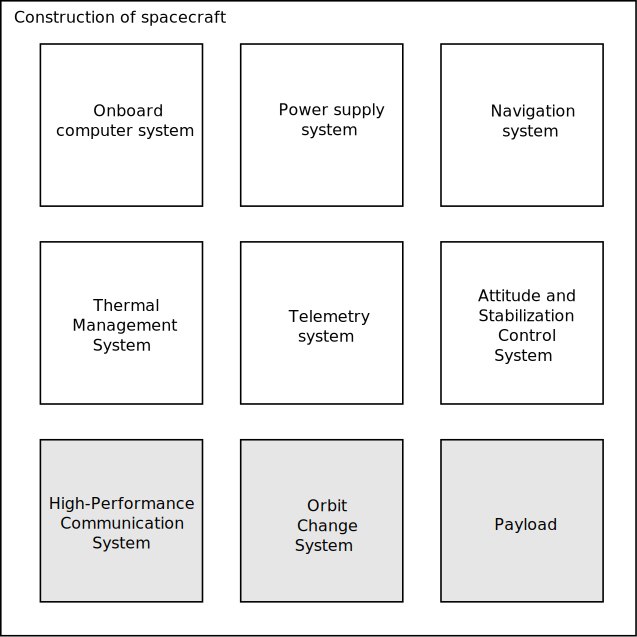
\includegraphics[width=12cm]{images/subsystems-en.eps}
    \caption{Diagram of spacecraft subsystems}
    \label{Pic:subsystems}
  \end{center}
\end{figure}

Each of the subsystems is characterized by the following set of parameters:

\begin{itemize}
\item weight (kg);
\item volume (l);
\item allowable temperature range: min./max. (°C);
\item power consumption (W);
\item heat dissipation (W);
\item current state (on, off, faulty).
\end{itemize}

Let us consider in more detail the purpose of each of the subsystems and their special parameters.
(\textbf{*}~--- mandatory subsystem):

\begin{description}
\item[Construction (body) of spacecraft (*)] The body makes up the outer contour of the spacecraft, and is also used for mounting all spacecraft systems. Special design options include:
   \begin{itemize}
     \item cube side size, m.
   \end{itemize}
\item[Onboard computer system (*)] Onboard computer system contains the main flight program and a set of service parameters. The special parameters of the Onboard computer system include:
   \begin{itemize}
     \item RAM, MB.
   \end{itemize}
\item [Power supply system (*)] The power supply system (PSS) provides electrical energy to all spacecraft systems. As a rule, this system consists of a battery and a set of solar panels, as well as a power management system. The special parameters of the PSS include:
   \begin{itemize}
   \item battery capacity, $\text{W} - \text{h}$;
   \item Efficiency of solar panels, \%;
   \item coefficient of heat absorption by solar panels;
   \item emissivity of solar panels.
   \end{itemize}

\item [Navigation system (*)] The navigation system contains a special computer and a set of sensors that allow you to determine the position of the spacecraft relative to the Earth with high accuracy. Has no special options.

\item [Attitude and Stabilization Control System (*)] The Attitude and Stabilization Control System ensures the orientation of the spacecraft in a given direction. The special parameters include:
   \begin{itemize}
     \item maximum moment, $\text{N} \cdot \text{m}$.
   \end{itemize}

\item [Thermal Management System (*)] The Thermal Management System is used to maintain the required temperature conditions of the spacecraft. Typically, this system contains temperature sensors, heaters, and a heatsink that can radiate excess heat into space. The Thermal Management System special parameters include:
   \begin{itemize}
   \item coefficient of heat absorption by radiators;
   \item heatsink emissivity;
   \item heater power, W.
   \end{itemize}

\item [Telemetry system (*)] The telemetry system is designed to transmit service messages to Earth about the state of the spacecraft and its systems. Typically, this system contains an independent low power transmitter. To the special parameters of the telemetry system
   relate:
   \begin{itemize}
   \item onboard antenna gain;
   \item ground antenna gain;
   \item antenna opening angle, °;
   \item transmitter power, W;
   \item frequency (MHz)
   \end{itemize}

\item [High-Performance Communication System] The high-performance communication system allows large amounts of data to be transmitted to Earth in short periods of time. The high performance communication system has the same special parameters as the telemetry system (see above).

\item [Orbit Change System] The orbit change system contains the propulsion system and fuel tanks.
   \begin{itemize}
     \item maximum mass fuel consumption, kg/s;
     \item specific impulse of the propulsion system, m/s;
     \item volume of fuel tanks, l.
   \end{itemize}

\item [Payload (option 1~--- camera)] The camera allows you to take digital pictures of objects on Earth and in space. Camera specific options include:
   \begin{itemize}
   \item field of view angle, °;
   \item spectral range;
   \item data stream, Mbit/s;
   \item memory size, MB;
   \item matrix, pix.
   \end{itemize}

\item [Payload (option 2~--- crystal container)] The container is designed for growing protein crystals and their subsequent transportation to Earth. The container contains heat-resistant walls, a parachute and a cushioning system during landing on Earth. The container has no special parameters.

\end{description}

A complete list of subsystems available for construction is presented in Appendix 1.

The body of the spacecraft is assumed to be cubic for ease of modeling, and bodies of various sizes are available. Thus, the spacecraft has six outer surfaces
(см. рисунок \ref{Pic:cube}).

\begin{figure}[tbh]
  \begin{center}
    % \includegraphics[width=6cm]{images/cube.eps}
    \caption{Principal spacecraft model}
    \label{Pic:cube}
  \end{center}
\end{figure}

The numbering of surfaces from 1 to 4 goes counterclockwise, surfaces 5 and 6 are in the X0Y plane, while surface 5 has a large coordinate along the Z axis. Taking into account the fact that in this model the spacecraft moves in the X-Y plane, faces 5 and 6 are always parallel to the plane of motion of the spacecraft.

The layout of the subsystem inside the spacecraft is not considered in the model, however, some subsystems have leads on the surface of the case:

\begin{itemize}
\item high-performance communication system antenna and payload (camera) are located on surface 1;
\item surfaces 1-4 can contain elements of solar panels and radiators; when designing, the ratio of the areas of solar panels, radiators and unoccupied surface~--– the same for all four surfaces;
\item surfaces 5-6 in this model are never illuminated by the Sun, so for them you can specify the ratio of the areas of radiators and the unoccupied surface~--– the same for both surfaces.
\end{itemize}

Also, the spacecraft can set the mass of fuel to be poured (kg). The fuel of a given mass must fit into the fuel tanks installed on the spacecraft (the volume of the tanks is determined in the parameters of the orbit change system). Regardless of the choice of engine used, a single type of fuel is used: \textbf{NTO+UDMH}, whose density is equal to \textbf{1185
  $\text{kg}/\text{m}^3$}.

When designing a spacecraft, the following restriction should also be taken into account: the maximum mass of a spacecraft should not exceed \textbf{20 tons}.

\section{Spacecraft simulation}

The spacecraft flight is simulated with a set or automatically selected time step. At each time step, an analysis of the interaction of blocks is carried out. At this stage, the simulator performs the following calculations:

\begin{enumerate}
   \item ballistic calculation (calculation of the position of the center of mass of the spacecraft);
   \item mechanical calculation (calculation of loads acting on the spacecraft and change of the spacecraft orientation under their action);
   \item energy calculation;
   \item thermal calculation;
   \item information exchange calculation;
   \item execution of flight programs;
   \item payload operation.
\end{enumerate}

\subsection{Ballistic calculation}
\label{Sec:Ballistics}

It is assumed in the model that the spacecraft flies around the Earth in the central gravitational field. The position of the spacecraft is described in a coordinate system, the origin of which is in the Earth's center of mass, the $x$ and $y$ axes are located in the orbit plane, the $z$ axis is replenished to the right triplet of vectors. The coordinate system is shown in the picture \ref{Pic:Coord}. The spacecraft flies in the plane of the $X0Y$ orbit.

\begin{figure}[tbh]
  \begin{center}
    \includegraphics[width=12cm]{images/coord-en.eps}
    \caption{Coordinate system in ballistic and mechanical calculations}
    \label{Pic:Coord}
  \end{center}
\end{figure}

The position of the spacecraft is measured by the navigation system without error.

At the initial moment of time, the spacecraft has coordinates equal to $(0, h_{\text{orb}} + R_{\text{E}},
0)$ where $h_{\text{orb}}$~--– the height of the initial orbit of the spacecraft, and $R_{\text{З}}$~-- is the radius of the Earth. At any time, the position of the spacecraft is set
$(X_{\text{SC}}, Y_{\text{SC}}, 0)$ or a pair from the angle of the spacecraft position $\alpha$ the initial value is 0, increases clockwise from the $y$ axis) and the current orbit height $h_{\text{orb}}$. The spacecraft is also characterized by the orientation angle $\varphi$ (the initial value of which is equal to 0, it increases counterclockwise from the $x$ axis). \textbf{All distances in the model are measured in meters (unless otherwise stated), angles~--- in degrees.}

The position of the Sun in this model is constant and equals $(+\infty, 0, 0)$. Accordingly, the same half of the Earth is illuminated.

The following three forces act on the spacecraft in flight:

\begin{itemize}
\item force of gravitational attraction to the Earth;
\item thrust force of the engine (if the engine is installed on the spacecraft and turned on);
\item aerodynamic drag force (if the spacecraft has reached the earth's atmosphere).
\end{itemize}

All forces also act only in the $X0Y$ orbital plane.

\paragraph{The force of gravitational attraction}

At an arbitrary point in time, the spacecraft is located at a point with coordinates $(X_{\text{SC}}, Y_{\text{SC}}, 0)$, while the force of gravitational attraction to the Earth $F_{\text {G}}$, see picture \ref{Pic:Gravity}.

\begin{figure}[tbh]
  \begin{center}
    \includegraphics[width=10cm]{images/gravity-en.eps}
    \caption{The position of the spacecraft in orbit and the direction of the force of gravitational attraction to the Earth}
    \label{Pic:Gravity}
  \end{center}
\end{figure}

The magnitude of the force is calculated according to the law of universal gravitation \ref{Eq:gravity}:

\begin{eqnarray}
  F_{\text{G}} = G \frac{m_{\text{SC}} M_{\text{E}}}{R_{\text{SC}}^2}, \label{Eq:gravity}
\end{eqnarray}

where $G$~--- gravitational constant, equal to $6,67384 \cdot 10^{-11} \text{m}^3
\text{kg}^{-1} \text{c}^{-2}$; $m_{\text{SC}}$~--- current spacecraft mass, kg; $M_{\text{E}}$~--–
the mass of the Earth, equal to $5,97 \cdot 10^{24} \text{kg}$; $R_{\text{SC}}$~--– the length of the radius vector of the spacecraft at the current time.

The value of the speed of the device when moving in orbit is calculated by the formula:

\begin{eqnarray}
  v_{\text{orb}} = \sqrt{\frac{G M_{\text{E}}}{R_{\text{E}} + h_{\text{orb}}}}, \label{Eq:orbital-velocity}
\end{eqnarray}

where $G$~--- gravitational constant, and $M_{\text{E}}$~--- mass of the Earth.

The length of the SC radius vector at the current time RSC can be calculated by the formula
\ref{Eq:radius-vector}:

\begin{eqnarray}
  R_{\text{SC}} = \sqrt{X_{\text{SC}}^2 + Y_{\text{SC}}^2}, \label{Eq:radius-vector}
\end{eqnarray}

The projections of the force of gravitational attraction $F_{\text{F}}$, indicated in the figure \ref{Pic:Gravity} on the axes of the coordinate system, can be written in the following form
(\ref{Eq:gravity-force}):

\begin{eqnarray}
  F_{\text{G}}^X = - G \frac{m_{\text{SC}} M_{\text{E}}}{\left(X_{\text{SC}}^2 +
    Y_{\text{SC}}^2\right)^{\frac{3}{2}}} X_{\text{SC}}, \nonumber \\
  F_{\text{G q}}^Y = - G \frac{m_{\text{SC}} M_{\text{E}}}{\left(X_{\text{SC}}^2 +
    Y_{\text{SC}}^2\right)^{\frac{3}{2}}} Y_{\text{SC}} \label{Eq:gravity-force}
\end{eqnarray}

\paragraph{Engine thrust}

A coordinate system is also connected with the spacecraft body, the reference point of which is located in the center of mass of the spacecraft. At the initial moment of time, the axes of the coordinate system are parallel to the axes of the Earth's coordinate system shown in the figure \ref{Pic:Coord}. In the absence of spacecraft rotation relative to its own center of mass, the axes of the coordinate systems remain parallel during the entire orbit, see figure \ref{Pic:Coord-Sat}.

\begin{figure}[tbh]
  \begin{center}
    \includegraphics[width=10cm]{images/coord-sat-en.eps}
    \caption{Mutual arrangement of coordinate systems of the Earth and spacecraft}
    \label{Pic:Coord-Sat}
  \end{center}
\end{figure}

The orientation of the spacecraft is given by the angle of rotation $\varphi$ (or $\varphi_Z$) of the $X_{\text{SC}}$ axis relative to the $X$ axis of the Earth's coordinate system, which corresponds to the rotation of the spacecraft about the $Z$ axis. The angle of rotation sets the direction of the plane of the device.

The direction of the thrust force of the engine is rigidly related to the direction of the $x_{\text{SC}}$ axis of the spacecraft coordinate system, which leads to the need to change the orientation of the spacecraft to change the direction of the thrust force. The state of the orbit correction system (OCS) is controlled by the control system. The amount of thrust is regulated discretely: either the OCS is turned on and creates thrust, or the OCS is turned off and does not create thrust.

The thrust value with the propulsion system turned on is calculated by the formula
\ref{Eq:traction-force}:

\begin{eqnarray}
  F_{\text{T}} = \Delta m I_{\text{si}}, \label{Eq:traction-force}
\end{eqnarray}

where $\Delta m$~--– mass consumption of fuel component, kg/s, $I_{\text{si}}$~---– specific impulse of the propulsion system, m/s.

It is obvious that the propulsion system can create thrust in the case when there is still fuel left in the tanks of the orbit change system. The dependence of the fuel mass $m_{\text{T}}$ on the operating time of the propulsion system $t_{\text{PS}}$ with the shaving change system on is as follows:

\begin{eqnarray}
  m_{\text{Т}} = m_{\text{T}}^0, - \Delta m t_{\text{PS}}
\end{eqnarray}

where $m_{\text{T}}^0$~--– the mass of fuel in the tanks of the orbit change system before switching on,
kg.

The projections of the thrust force on the axes of the Earth's coordinate system can be written in the following form
(\ref{Eq:traction-force-proj}):

\begin{eqnarray}
  F_{\text{T}}^X = \Delta m I_{\text{si}} \cos{\varphi_Z} \nonumber \\
  F_{\text{T}}^Y = \Delta m I_{\text{si}} \sin{\varphi_Z} \label{Eq:traction-force-proj}
\end{eqnarray}

\paragraph{Aerodynamic Drag Force}

The aerodynamic drag force FA arises when the spacecraft moves in the upper atmosphere, the force value is calculated by the formula \ref{Eq:stokes}:

\begin{eqnarray}
   F_{\text{A}} = C_\xi \frac{\rho V_{\text{SC}}^2}{2} S_{\text{SC}}, \label{Eq:stokes}
\end{eqnarray}

where $C_\xi$~-- is the aerodynamic drag coefficient of the spacecraft, equal to $1.05$ (value for the cube); $\rho$~--– atmospheric density at current spacecraft flight altitude\footnote{See GOST 4401-81~--— The atmosphere is standard. Parameters, for example in Wikipedia}, $\text{kg}/\text{m}^3$; $V_{\text{SC}}$~--– current spacecraft flight speed, m/s; $S_{\text{SC}}$~--- SC cross-sectional area, $\text{m}^2$. The aerodynamic drag force $F_{\text{A}}$ is directed opposite to the spacecraft velocity vector, see figure \ref{Pic:Stokes}.

\begin{figure}[tbh]
  \begin{center}
    \includegraphics[width=10cm]{images/stokes-en.eps}
    \caption{Direction of the aerodynamic drag force $F_{\text{A}}$ and its projections on the axes of the coordinate system associated with the Earth}
    \label{Pic:Stokes}
  \end{center}
\end{figure}

To calculate the projections of the aerodynamic drag force on the axes of the coordinate system associated with the Earth, $F_{\text{A}}^X$ and $F_{\text{A}}^Y$, we use the decomposition of the velocity into projections (formula \ref{ Eq:velocity-vector}).

\begin{eqnarray}
  V_{\text{SC}}^2 = \left( V_{\text{SC}}^X \right)^2 + \left( V_{\text{SC}}^Y \right)^2
  \label{Eq:velocity-vector}
\end{eqnarray}

and then the projections corresponding to the picture \ref{Pic:Stokes} are calculated by the formulas
\ref{Eq:stokes-proj}:

\begin{eqnarray}
  F_{\text{A}}^X = - C_\xi \frac{\rho \left| V_{\text{SC}}^X \right| V_{\text{SC}}^X}{2} S_{\text{SC}} \nonumber \\
  F_{\text{A}}^Y = - C_\xi \frac{\rho \left| V_{\text{SC}}^Y \right| V_{\text{SC}}^Y}{2} S_{\text{SC}} \label{Eq:stokes-proj}
\end{eqnarray}

\paragraph{Integration of equations of motion of the center of mass SC}

A complete set of equations of motion is obtained by substituting the equations for the force projections \ref{Eq:gravity}, \ref{Eq:traction-force} and \ref{Eq:stokes} into the equation of Newton's second law, written for two projections on the axes of the coordinate system, associated with the earth:

\begin{eqnarray}
   m_{\text{SC}} \cdot a_{\text{SC}}^X = F_{\text{T}}^X + F_{\text{T}}^X + F_{\text{A} }^X
   m_{\text{SC}} \cdot a_{\text{SC}}^Y = F_{\text{T}}^Y + F_{\text{T}}^Y + F_{\text{A} }^Y
\end{eqnarray}

The motion of the spacecraft's center of mass can be simulated using a special ballistic calculator (see the section \ref{Sec:Calculator}).

\subsection{Mechanical calculation}
\label{Sec:Mechanics}

At the initial time $t_0 = 0$ the spacecraft has an angular velocity $\omega_0 = 1\degree/\text{c}$ about the $Z$ axis. The angular velocity of the apparatus varies according to the formula:

\begin{eqnarray}
  \omega(t) = \omega_0 + \varepsilon t,
\end{eqnarray}

where $\varepsilon$~-- is the angular acceleration of the craft, $\degree/\text{c}^2$.

The angular velocity and attitude angle of the spacecraft are measured by the attitude control system without error. The change in the orientation angle of the spacecraft is determined by the formula:

\begin{eqnarray}
   \varphi(t) = \varphi_0 + \omega t + \frac{\varepsilon t^2}{2},
\end{eqnarray}

where $\varphi_0$~--- the starting orientation of the spacecraft.

Changing the orientation of the spacecraft is done using a flywheel engine or other spacecraft\footnote{In the current version of the manual, only the flywheel model is considered.}, which is part of the attitude control and stabilization system. It is believed that the flywheel does not have a limiting rotation speed, so there is no need to carry out the operation of resetting the accumulated kinetic moment.

Taking into account the described assumptions, the equation describing the rotational dynamics of the spacecraft can be written as (formula \ref{Eq:flywheel}):

\begin{eqnarray}
  I_z \varepsilon = M_Z(t) \label{Eq:flywheel}\\
  \varepsilon = \frac{M_Z}{I_Z}, \label{Eq:angular-acceleration}
\end{eqnarray}

where $I_Z$~--- moment of inertia of the spacecraft during rotation about the $Z$ axis, $\text{kg} \cdot \text{m}^2$; $M_Z(t)$~--- moment generated by the flywheel motor relative to the $Z$ axis, $\text{Н} \cdot \text{m}$. The moment can be set by the flight program within the limits allowed for a given engine-flywheel.

In this model, the SC is a cube of a given size. We believe that the mass of the spacecraft is distributed evenly over its volume, so the moment of inertia of the spacecraft is calculated as follows:

\begin{eqnarray}
   I_z = \frac{1}{12} (2 a^2) m(t), \label{Eq:inertia-moment}
\end{eqnarray}

where $a$~-- is the size of the spacecraft face, m; $m(t)$~--- the mass of the spacecraft at time $t$.

The rotation of the spacecraft around the center of mass can be simulated using a special mechanical calculator (see section \ref{Sec:Calculator}).

\subsection{Energy calculation}
\label{Sec:Energy}

At each moment of time, the spacecraft is characterized by $P_{\text{consum}}$ consumed and $P_{\text{gen}}$ generated by power. The power consumption is the sum of the consumption of all enabled devices (which are in the \verb'ON' state):

\begin{eqnarray}
   P_{\text{consum}} = \sum_i{P_{i}^{ON}}
\end{eqnarray}

The generated power is the sum of the current generated by the solar panels~--– photovoltaic cells~--- and the current supplied from the battery.

\begin{eqnarray}
  P_{\text{gen}} = P_{\text{PV}} + P_{\text{acc}}
\end{eqnarray}

Photovoltaic cells (PV cells) are located on the side faces of the device (1-4). It is believed that the sun illuminates one of the faces. The electrical power generated by the PV sells,
is calculated as follows (\ref{Eq:photoelement} formula):

\begin{eqnarray}
  P_{\text{PV}} = \eta_{\text{PV}} \cdot S_{\text{PV}} \cdot q_{\text{C}}(t), \label{Eq:photoelement}
\end{eqnarray}

where $\eta_{\text{PV}}$~--- PV efficiency; $S_{\text{PV}}$~--- total PV area on the illuminated face of the spacecraft, $\text{m}^2$; $q_{\text{С}}(t)$~--– solar radiation flux density, $\text{W} \cdot \text{m}^{-2}$, which is determined depending on the position of the spacecraft in orbit (see figure \ref{Pic:Coord}) according to the formula \ref{Eq:sunlight}:

\begin{eqnarray}
   q_{\text{С}}(t) = \left\{
   \begin{array}{l}
     0, \text{at}~X_{\text{SC}}(t) < 0~\text{u}~|Y_{\text{SC}}(t)| \leqslant R_{\text{E}}\\
     1400, \text{ in all other cases.}
   \end{array}
\right. \label{Eq:sunlight}
\end{eqnarray}

It is believed that for any orientation of the spacecraft, the Sun will illuminate an area equal to the area of the solar panels located on the side surface of the body (1-4). The PV area is determined by the formula:

\begin{eqnarray}
   S_{\text{PV}} = k^{(1-4)}_{\text{fsp}} \cdot a^2, \label{Eq:photopanels}
\end{eqnarray}

where $k^{(1-4)}_{\text{fsp}}$~--- is the fraction of solar panels on each of the surfaces 1-4 of the spacecraft (design parameter), $a$~-- is the length of the spacecraft face, m. The onboard chemical storage battery is characterized by the capacity, $\text{W}-\text{h}$. Possible the following options:
$$
  \left\{
   \begin{array}{l}
     P_{\text{consum}} < P_{\text{gen}}, \text{excess electricity charges
       battery};\\
     P_{\text{consum}} = P_{\text{gen}}, \text{battery not in use};\\
     P_{\text{consum}} > P_{\text{gen}}, \text{solar current is not enough,
       battery in use}.\\
   \end{array}
\right.
$$

The battery compensates for the consumption of the device if the current generated by the solar panels is not enough for operation. If the generated current exceeds the consumed, the battery can be recharged. Excess electricity that did not go to charge the battery is discharged to the resistor, i.e. are ignored.

\paragraph{Power shortage}

Separate consideration requires the case of shortage of electricity. If the spacecraft subsystems consume more energy than the power supply subsystem can supply, the spacecraft goes into power saving mode (\verb'SAFE MODE'), in which only three subsystems remain on: the power supply system itself, the on-board computer system and the telemetry subsystem, the remaining subsystems turn off. In this case, the onboard computer system switches to the \verb'STATE_SAFE' mode. The transition to the normal operation mode of the device is carried out by changing the operation mode of the onboard computer system to \verb'STATE_WAKEUP' (see section \ref{Sec:CPU}). If there is a shortage of electricity already in the power saving mode, the spacecraft fails.

\subsection{Thermal calculation}
\label{Sec:Heat}

We assume that in the simulated spacecraft individual blocks of equipment are connected by thermal links with low thermal resistance, which leads to the equalization of the temperature field throughout the spacecraft. In other words, the spacecraft temperature is characterized by a single value~--– $T$, K. The spacecraft temperature $T$ affects the operation of spacecraft. Each subsystem has two characteristics: the minimum and maximum allowable temperatures. When crossing
either of the two boundaries subsystem fails \emph{note that the temperature regime of the subsystems is set in degrees Celsius, and this model and telemetry of the device operates in Kelvins}).

The spacecraft temperature $T$ varies with time as follows (formula \ref{Eq:temperature}):
\begin{eqnarray}
c \cdot m(t) \cdot \frac{\Delta T}{\Delta t} = Q^{\Sigma}_{\text{outer}} + Q^{\Sigma}_{\text{inner}}, \label{Eq:temperature}
\end{eqnarray}

where $c$~--- average specific heat of spacecraft materials, equal to \textbf{800 $\text{J}
   \cdot \text{kg}^{-1} \cdot \text{K}^{-1}$}; $m(t)$~--– spacecraft mass at time $t$;
$Q^{\Sigma}_{\text{outer}}$~--- term describing the external heat transfer of the spacecraft;
$Q^{\Sigma}_{\text{inner}}$~--– the sum of heat releases from onboard equipment subsystems in time $t$.

External heat exchange is calculated for the entire surface of the device as shown in the figure \ref{Pic:heat-exchange}.

\begin{figure}[tbh]
  \begin{center}
    \includegraphics[width=7cm]{images/heat-exchange.eps}
    \caption{External heat exchange spacecraft}
    \label{Pic:heat-exchange}
  \end{center}
\end{figure}

It is believed that one face of the spacecraft (one of the surfaces 1-4), closest to the Sun, is heated by the heat flux. When designing the spacecraft, the ratio of the areas of solar panels, radiator and heat insulator is indicated, since they heat up differently: the heat absorption coefficient for solar panels and the radiator is indicated in the parameters of subsystems, and for the heat insulator it is 0.

At the same time, all facets of the device radiate heat. Solar panels and radiators have different degrees of emissivity specified in the subsystem parameters, and the blackness of the heat insulator
considered to be 0.

Thus, the external heat exchange of the spacecraft is calculated by the formula \ref{Eq:heat-exchange}:

\begin{eqnarray}
  Q^{\Sigma}_{\text{outer}} = \left(S_{\text{sp}}^{\text{absorption}} A_{\text{sp}} +
  S_{\text{rad}}^{\text{absorption}} A_{\text{rad}}\right) \cdot q_{\text{C}}(t) -
  \left(S_{\text{sp}}^{\text{est}} \varepsilon_{\text{sp}} + S_{\text{rad}}^{\text{est}}
  \varepsilon_{\text{rad}}\right)
  \sigma T^4, \label{Eq:heat-exchange}
\end{eqnarray}

where $S_{\text{sp}}^{\text{absorption}}$~--- area of heat absorption by solar panels,
$\text{m}^2$; $A_{\text{sp}}$~--– absorption coefficient of solar radiation by solar
batteries; $S_{\text{sp}}^{\text{absorption}}$~--– area of heat absorption from the sun
radiators, $\text{m}^2$; $A_{\text{sp}}$~--– solar absorption coefficient
radiators; $q_{\text{С}}(t)$~--– solar radiation flux density, $\text{W} \cdot
\text{m}^{-2}$ which was previously defined in \ref{Eq:sunlight};
$S_{\text{sp}}^{\text{est}}$~--- radiation area of the spacecraft solar panels, $\text{m}^2$; $\varepsilon_{\text{sat}}$~--–
degree of blackness of solar panels; $S_{\text{rad}}^{\text{est}}$~--– radiation area
all spacecraft radiators, $\text{m}^2$; $\varepsilon_{\text{rad}}$~--– heatsink emissivity; $\sigma$~--- constant in law
Stefan-Boltzmann equal to $5.67 \cdot 10^{-8} \cdot \text{J} \cdot \text{c}^{-1} \cdot
\text{m}^{-2} \cdot \text{K}^{-4}$.

\begin{figure}[tbh]
   \begin{center}
     % \includegraphics[width=15cm]{images/surfaces.eps}
     \caption{Location of solar panels and radiators on the sides of the device}
     \label{Pic:surfaces}
   \end{center}
\end{figure}

The required areas are calculated as follows:

\begin{eqnarray}
   \begin{array}{l}
   S_{\text{sp}}^{\text{abs}} = k^{(1-4)}_{\text{sp}} \cdot a^2 \\
   S_{\text{rad}}^{\text{adv}} = k^{(1-4)}_{\text{rad}} \cdot a^2 \\
   S_{\text{sp}}^{\text{est}} = 4 \cdot k^{(1-4)}_{\text{sp}} \cdot a^2 \\
   S_{\text{rad}}^{\text{est}} = (4 \cdot k^{(1-4)}_{\text{est}} + 2 \cdot
   k^{(5-6)}_{\text{rad}} \cdot a^2
   \end{array}
\end{eqnarray}

where $a$~--- the size of the edge of the spacecraft, m; $k^{(1-4)}_{\text{sp}}$~--- the fraction of the area of solar panels on each
surfaces 1-4; $k^{(1-4)}_{\text{rad}}$~--- area fraction of radiators on each surface 1-4; $k^{(5-6)}_{\text{rad}}$~--- area fraction of radiators on each surface 5-6.

When designing the spacecraft, it is necessary to specify the share of solar panels and radiators on faces 1-4 and the share of radiators on faces 5-6. The rest of the surface is covered with a special film that prevents heat transfer (see Fig. \ref{Pic:surfaces}).

The mass of solar panels and radiators can be neglected.

The sum of heat releases of the spacecraft subsystems is calculated only for the included subsystems according to the formula
\ref{Eq:heat_prod}:

\begin{eqnarray}
Q^{\Sigma}_{\text{inner}}(t) = \sum_i Q_{i}^{ON}(t), \label{Eq:heat_prod}.
\end{eqnarray}

The thermal management subsystem of the spacecraft has additional heaters that can be turned on in the flight program. Thus, the spacecraft can be additionally heated from the inside, if this
will be necessary.

\subsection{Information exchange calculation}
\label{Sec:Radio}

The spacecraft enters into information exchange with one or more ground control complexes via radio communication. Let us assume that the connection between the spacecraft and the Earth is arranged in the same way in both directions (from the spacecraft to ground station or vice versa). The ground station coordinates are given in the conditions for solving the problem. We will assume that the ground station antenna constantly tracks the trajectory of the spacecraft.

The onboard antenna of the spacecraft is fixed fixedly on the body of the spacecraft (on surface 1) and has a radiation pattern with an opening angle specified in the parameters of the transmitting
antennas. The radiation pattern of the onboard antenna is located in such a way that it is divided in half by the spacecraft orientation vector (see figure \ref{Pic:Radio}). There are antennas with a 360° opening angle.

The antenna signal is shielded by the ground.

\begin{figure}[tbh]
  \begin{center}
    % \includegraphics[width=12cm]{images/radio.eps}
    \caption{SC antenna directivity}
    \label{Pic:Radio}
  \end{center}
\end{figure}

The signal power $P_2$ at the input to the ground station receiver is calculated by the formula
\ref{Eq:gs-signal}:

\begin{eqnarray}
P_2 = \frac{G_1 G_2 \Delta_2 P_1}{b_1 b_2 L_{12}}, \label{Eq:gs-signal}.
\end{eqnarray}

where $P_1$~--- SC transmitter power, W; $G_1$ and $G_2$~--– gains onboard and ground
antennas that depend on the antenna type and are specified in the subsystem parameters; $b_1$ and $b_2$~--–
losses in the onboard and ground radio path (we assume that $b_1 = 1$ and $b_2 = 1$);
$\Delta_2$~--– losses due to inaccurate pointing of the receiving antenna at the spacecraft (we assume that
there are no losses and $\Delta_2 = 1$); $L_{12}$~--– signal weakening on the way from the spacecraft to
GS calculated using the formula \ref{Eq:signal-attenuation}:

\begin{eqnarray}
L_{12} = \left( \frac{4 \pi L_{\text{GS}}}{\lambda_1} \right)^2 \Delta L_{12}, \label{Eq:signal-attenuation}.
\end{eqnarray}

where $L_{\text{GS}} = \sqrt{(X_{\text{GS}} - X_{\text{SC}})^2 + (Y_{\text{GS}} -
  Y_{\text{SC}})^2 + (Z_{\text{GS}} - Z_{\text{SC}})^2}$~--- SC distance to GS, m (recall that in this model the coordinate $ Z = 0$); $\lambda_1$~--- transmitter wavelength (calculated using the transmission frequency specified in the subsystem parameters); $\Delta L_{12}$~--- losses due to non-ideal medium (we assume that there are no losses and $\Delta L_{12} = 1$). If the GS is not in the beam pattern of the transmitting antenna, $G_1 = 0$.

The radio channel uses phase modulation with quadruple keying. Noise power
at the input to the receiver, the GS P2Ш is calculated by the formula \ref{Eq:noise}:

\begin{eqnarray}
P_{2\text{N}} = k T_2 \Delta f_k, \label{Eq:noise}
\end{eqnarray}

where $k = 1.38 \cdot 10^{-23}$~--- Boltzmann constant, $\text{W} \cdot \text{Hz}^{-1}
\cdot \text{K}^{-1}$; $T_2 = 1000$~--- receiver noise temperature, K; $\Delta f_k$~--- band
communication channel frequency, Hz, which is calculated by the formula \ref{Eq:freq}:

\begin{eqnarray}
\Delta f_k = \frac{1,2 R}{\log_2{M}}, \label{Eq:freq}
\end{eqnarray}

where $R$~--- information transfer rate, bit/s; $M = 4$~--– multiplicity of phase manipulation. The signal-to-noise ratio during a communication session should not fall below 100:

\begin{eqnarray}
\frac{P_{2}}{P_{2\text{N}}} \geqslant 100 \label{Eq:signal-noise}
\end{eqnarray}

By substituting \ref{Eq:gs-signal}-\ref{Eq:freq} into the \ref{Eq:signal-noise} condition, you can get the width of the information transmission channel (bits) for a given position of the spacecraft in orbit, the orientation of the spacecraft and on-board transmitter power:

\begin{eqnarray}
R = \frac{1}{100} \frac{G_1 G_2 P_1}{\left( \frac{4 \pi L_{\text{GS}}}{\lambda_1}
  \right)^2} \left( \frac{\log_2{M}}{1,2 R \cdot k \cdot T_2} \right)
\end{eqnarray}

\paragraph{Types of communication devices}

In the current spacecraft architecture, two subsystems contain a receiver, a transmitter, and the corresponding antennas. The first~--- obligatory subsystem~--- is the \textbf{telemetry subsystem}, which serves to transmit messages about the state of the spacecraft and its subsystems to the Earth. Such transmissions can be received by any GS on the surface of the Earth. As a rule, the telemetry system is equipped with a VHF transmitter with an omnidirectional antenna and low bandwidth.

The second subsystem~--- \textbf{high-performance communication}, which can be installed if necessary, is used to transmit large messages, such as images. If necessary, SC messages can only be directed to a specific GS, then these messages are ignored by other GSs.

It is believed that a message acceptance acknowledgment system is used. Until the message is fully received by the recipient (SC), the next message will not be sent.

Communication devices are equipped with RAM for storing messages. When the RAM is exhausted, new messages do not enter the queue of transmitted messages.

\subsection{Flight control}
\label{Sec:CPU}

All subsystems of the spacecraft, except for the body, are characterized by a state at any time. The state or mode of a subsystem can take the following values:

\begin{itemize}
\item \verb'STATE_OFF'~--- subsystem is off; in this case, it does not consume electricity, does not generate heat, does not generate data flow, does not execute the program;
\item \verb'STATE_ON'~--- subsystem enabled; if the subsystem has a flight program (like an on-board computer), it will be continuously executed; the subsystem begins to consume electricity and heat up; in this case, it performs its specific function, which differs for different subsystems:
    \begin{description}
   \item[power system] produces electricity; disabling this power subsystem puts the spacecraft into power saving mode (\verb'SAFE MODE').
   \item[navigation system] obtains the spacecraft's position using sensors and provides this data to flight programs;
   \item[attitude and stabilization control system] obtains the attitude of the spacecraft using sensors and provides this data to flight programs, and also makes it possible to use attitude change devices (flywheels, etc.);
   \item[thermal management system] receives information about the temperature inside the spacecraft; starts cooling the spacecraft through the radiator; allows you to turn on the heater;
   \item[telemetry system] receives data from all systems and tries to send the accumulated data from the buffer to Earth;
   \item[high-performance communication system] attempts to send all data in the buffer to Earth sequentially;
   \item[payload system] depending on payload type:
     \begin{itemize}
       \item \emph{camera}~--- allows you to control the camera;
       \item \emph{container for growing protein crystals}~--- allows you to start growing crystals;
     \end{itemize}
   \item[orbit change system] obtains data on the available mass of propellant, allows
     turn on the engine, control traction;
   \end{description}
\item \verb'STATE_SLEEP'~--- subsystem is in sleep mode; in this state, it does not radiate heat and consumes 0.1 W of electricity;
\item \verb'STATE_DEAD'~--– subsystem failed; the operation of this system is impossible until the end of the flight;
\item \verb'STATE_SAFE'~--– this mode can only be accepted by the central computer; in this case, the spacecraft is in power saving mode (\verb'SAFE MODE'). Exit from this mode of operation is possible only by changing the mode of the central computer.
\end{itemize}

Some subsystems of the spacecraft are equipped with their own computing systems and can be separately programmed before the start of the flight.

In the current version of the simulator, no spacecraft program can be changed during the flight.

The subsystem program runs under the following conditions:

\begin{itemize}
\item subsystem is enabled (set to \verb'STATE_ON');
\item subsystem program contains no syntax errors.
\end{itemize}

For programming subsystems, the Python language is used, which is described in detail in a separate manual (see Appendix 2), and hierarchical state machine diagrams, which are described in a separate manual.

\subsection{Payload operation}
\label{Sec:Load}

There are three types of payload:

\begin{enumerate}
\item creation of protein crystals in weightlessness (mission "Protein crystal");
\item acquisition of images (missions "RS" and "Satellite Inspection");
\item in other missions (“Communication with the Earth” and “SMS everywhere”), the role of the payload is actually played by a high-performance communication system (in this case, the device does not have
   special \emph{payload} subsystem).
\end{enumerate}

The first type of payload does not imply any special modeling. The operating conditions necessary for the correct operation of this spacecraft are specified in the mission description.

Consider modeling the process of obtaining images using a camera. The camera is installed on the spacecraft in such a way that its axis coincides with the direction of the spacecraft's orientation - on surface 1 (see figure \ref{Pic:Camera-Orbit}).

\begin{figure}[tbh]
  \begin{center}
    \includegraphics[width=12cm]{images/camera-orbit.eps}
    \caption{Position of spacecraft and direction of photography}
    \label{Pic:Camera-Orbit}
  \end{center}
\end{figure}

The spacecraft orientation is characterized by the angle $\varphi$. The camera is located on surface 1, so it is directed at the same angle.

The camera is controlled through special commands in the flight program. It is possible to take a single shot or shoot a stream of frames. The image taken by the camera must be completely transmitted to Earth via a high-performance communication channel. The higher the resolution of the target image, as well as the deviation from the target ($\theta$) and, in the case of remote sensing, the normality of the satellite with respect to the surface ($\beta$), the higher the scores received for the image.

\begin{figure}[tbh]
  \begin{center}
    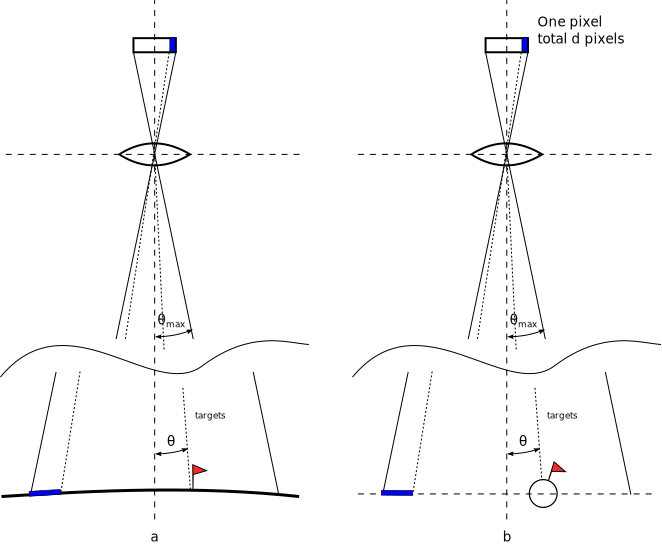
\includegraphics[width=14cm]{images/camera-en.eps}
    \caption{Spacecraft camera parameters}
    \label{Pic:Camera}
  \end{center}
\end{figure}

The figure \ref{Pic:Camera} shows the parameters that must be taken into account when shooting an object on the Earth (a) and in space (b) with a camera.

The angle $\theta_{\text{max}}$ (°)~--- is the angle of the camera's field of view, the angle $\theta$ (°)~--- is the angle of the target deviation from the shooting axis, which should not exceed the angle field of view, otherwise the object will not be captured. The camera resolution $d$~-- is the size of the matrix in pixels (we consider the matrix to be one-dimensional), which is given in the camera parameters. Then the image resolution $D$ (m/pixels) is obtained by the formula \ref{Eq:resolution}:
\begin{eqnarray}
  D = \frac{2 \cdot r_{\text{target}}\cdot \cos{\theta}\tan{\left(\theta_{\text{max}}\right)}}{d} =
  \frac{2 \cdot r \cdot \tan{\left(\theta_{\text{max}}\right)}}{d},
  \label{Eq:resolution}
\end{eqnarray}

where $r_{\text{target}}$~-- is the distance from the spacecraft to the target, m; $r$~--— optical distance
axes, m (in the case of remote sensing, equal to the altitude of the spacecraft orbit).

The normal orientation of the device also affects the image quality (see figure
\ref{Pic:Camera-Angle}).

\begin{figure}[tbh]
  \begin{center}
    \includegraphics[width=15cm]{images/camera-angle.eps}
    \caption{Various options for the normal orientation of the spacecraft in relation to the target}
    \label{Pic:Camera-Angle}
  \end{center}
\end{figure}

Even if there is no deviation from the target when shooting, the more normally the spacecraft is oriented, the better the picture of the object will turn out. In the case of shooting an object in space (“Satellite Inspection” mission), the same formula is applied, while the distance to the target is ~--- this is the distance between the spacecraft and the object being photographed.

Another important parameter of the camera is ~--- the amount of RAM of the computer system. When shooting starts, the data stream begins to continuously enter the memory of the computer system. The picture is sent to the radio channel after the end of shooting. If the RAM of the camera's computing system becomes full, the existing image is discarded (so you can lose a good shot).

\section{Means for solving the problem}

\subsection{Flight telemetry}
\label{Sec:Telemetry}

To analyze the flight, it is recommended to carefully study the telemetry data. The telemetry of the spacecraft is presented in the form of graphs and in the form of detailed textual information.

\textbf{Important:} at the end of the mission, you will see only those telemetry messages (and graphs based on them) that were transmitted to Earth. Below is an example of a single telemetry message. Please note that the time of receiving the telemetry signal may not coincide with the time of the event (the telemetry data arrives on Earth later).

\begin{verbatim}
05:10:41: [C:+:t=0017820][P:+:G=098.0:C=037.7:A=926472.0+]
  [R:+:B=00.0000:Q=00.7500]
  [N:+:X=05046958.7:Y=05080060.5:H=789.89:V=7460.80:Acc=7.774:A=44.81:DS=-]
  [E:-][O:+:OA=149.00:w=-00.000][T:+:B=0000.00:Q=000001][H:+:T=285.2][L:-]
05:10:41: [C:+:t=0017880][P:+:G=098.0:C=037.7:A=930090.0+]
  [R:+:B=00.0000:Q=00.7500]
  [N:+:X=05354427.6:Y=04754810.0:H=789.84:V=7460.85:Acc=7.774:A=48.39:DS=-]
  [E:-][O:+:OA=149.00:w=-00.000][T:+:B=0000.00:Q=000001][H:+:T=285.3][L:-]
05:10:41: [C:+:t=0017940][P:+:G=098.0:C=037.7:A=933120.0]
  [R:+:B=00.0000:Q=00.7500]
  [N:+:X=05640977.6:Y=04410983.2:H=789.79:V=7460.91:Acc=7.774:A=51.98:DS=-]
  [E:-][O:+:OA=149.00:w=-00.000][T:+:B=0000.00:Q=000001][H:+:T=285.5][L:-]
05:10:41: [C:+:t=0018000][P:+:G=098.0:C=037.7:A=933120.0]
  [R:+:B=00.0000:Q=00.7500]
  [N:+:X=05905488.7:Y=04049923.0:H=789.74:V=7460.96:Acc=7.774:A=55.56:DS=-]
  [E:-][O:+:OA=149.00:w=-00.000][T:+:B=0000.00:Q=000001][H:+:T=285.6][L:-]
...
\end{verbatim}

The telemetry line contains the time of receiving a signal from the device and information about the status of all subsystems. Each subsystem is characterized by a name (letter) and has a state that
denoted by the following symbols:

\begin{itemize}
\item \verb'0' subsystem is missing from the device;
\item \verb'+' subsystem enabled (state \verb'STATE_ON');
\item \verb'-' subsystem is off (state \verb'STATE_OFF');
\item \verb's' subsystem is in sleep state (state \verb'STATE_SLEEP');
\item \verb'x' subsystem is out of order, for example due to overheating (state
   subsystems \verb'STATE_DEAD');
\item \verb'S' subsystem is in power save mode (\verb'SAFE MODE').
\end{itemize}

Special parameters of subsystems are described in the table:

\begin{center}
\begin{longtable}{ |c|p{5cm}|p{9cm}| }
  \hline
  \textbf{Code} & \textbf{Subsystem name} & \textbf{Special Options} \\
  \hline
  \endhead
  \verb'C' & Onboard computer system &
  \begin{tabular}{p{8cm}}
    $t$~--– time from the start of the flight, s
  \end{tabular}\\
  \hline
  \verb'P' & Power supply system &
  \begin{tabular}{p{8cm}}
    \verb'G'~--- electricity generation, W;\\
    \verb'C'~--- electricity consumption, W;\\
    \verb'A'~--- energy stored in the battery, Wh;\\
  \end{tabular}\\
  \hline
  \verb'N' & Navigation system &
  \begin{tabular}{p{8cm}}
    \verb'X'~--– coordinate along the $X$ axis, m;\\
     \verb'Y'~--– coordinate along the $Y$ axis, m;\\
     \verb'H'~--– spacecraft orbit altitude, km;\\
     \verb'V'~--– vehicle speed, m/s;\\
     \verb'Acc'~--– total acceleration experienced by the vehicle, m/s2;\\
     \verb'A'~--– position angle of the spacecraft, °;\\
     \verb'DS'~--– flag for finding the spacecraft on the dark/light side;
  \end{tabular}\\
  \hline
  \verb'O' & Attitude and Stabilization Control System&
  \begin{tabular}{p{8cm}}
    \verb'OA'~--– spacecraft orientation angle, °;\\
    \verb'w'~--– spacecraft angular velocity,°/с;
  \end{tabular}\\
  \hline
  \verb'H' & Thermal management system &
  \begin{tabular}{p{8cm}}
    \verb'T'~--– spacecraft temperature, K;
  \end{tabular}\\
  \hline
  \verb'T' & Telemetry system &
  \begin{tabular}{p{8cm}}
    \verb'B'~--– transmission channel width, MB/s;\\
     \verb'Q'~--– message queue size, MB.
  \end{tabular}\\
  \hline
  \verb'R' & High performance communication system &
  \begin{tabular}{p{8cm}}
\verb'B'~--– transmission channel width, MB/s;\\
     \verb'Q'~--– message queue size, MB.
  \end{tabular}\\
  \hline
  \verb'E' & Orbit change system &
  \begin{tabular}{p{8cm}}
    \verb'F'~--- mass of available fuel, kg
  \end{tabular}\\
  \hline
  \verb'L' & Payload & none\\
  \hline
\end{longtable}
\end{center}

Telemetry results are also presented in the form of graphs (see figure
\ref{Pic:Telemetry}).

\begin{figure}[tbh]
  \begin{center}
    \includegraphics[width=15cm]{images/telemetry.eps}
    \caption{An example of telemetry graphs of the device after the mission}
    \label{Pic:Telemetry}
  \end{center}
\end{figure}

\subsection{Working with the ballistic-mechanical calculator}
\label{Sec:Calculator}

Within our simulation, each run of the simulator is equivalent to a real run. In order to calculate all the launch parameters, it is necessary to do a lot of preparatory work. To do this, you will be provided with the following tool: \textbf{ballistic-mechanical calculator}.

This program allows you to enter the initial state of the spacecraft, as well as control actions in order to obtain a change in the parameters of the spacecraft over time.

The ballistic calculator accepts the following parameters as input:

\begin{itemize}
\item size of the edge of the spacecraft side $(a)$, m;
\item initial weight of the spacecraft $(m)$, kg;
\item SC initial coordinates $(X_{\text{SC}}; Y_{\text{SC}})$, m;
\item SC initial velocity components $(V^X_{\text{SC}}; V^Y_{\text{SC}})$, m/s;
\item initial orientation angle of the spacecraft $(\varphi)$, °;
\item initial rotation speed of the spacecraft $(\omega)$, °/s;
\item control torque $(M)$, $\text{Н} \cdot \text{m}$;
\item duration of calculated flight $(d)$, s;
\item frequency of printing flight parameters $(t_p)$, s.
\end{itemize}

You can also enter an optional set of parameters that describe the operation of the engine:

\begin{itemize}
\item pulse on time $(t_e)$, s;
\item impulse duration $(d_e)$, s;
\item engine mass flow $(\Delta m)$, kg/s;
\item engine specific impulse $(I_{\text{si}})$, m/s.
\end{itemize}

The result of the calculation will be a set of data and graphs, similar to the output of the simulator.

The calculator can be found on the simulator's website. The results of running the calculator contain graphs and a sequence of values that looks like this:

\begin{verbatim}
Ti=00:00:00 X=00000994.0 Y=06931031.9 H=000560.0 Vx=9940.0 Vy=-0000.8
  A=000.0 Acc=008.3 As=000.0 m=0001.00 OA=360.0 w=00.0
Ti=00:00:10 X=00101385.9 Y=06930596.1 H=000560.3 Vx=9939.4 Vy=-0084.6
  A=000.8 Acc=008.3 As=000.0 m=0001.00 OA=360.0 w=00.0
Ti=00:00:20 X=00199777.9 Y=06929347.6 H=000561.2 Vx=9937.6 Vy=-0166.7
  A=001.6 Acc=008.3 As=000.0 m=0001.00 OA=360.0 w=00.0
Ti=00:00:30 X=00299140.0 Y=06927261.6 H=000562.7 Vx=9934.6 Vy=-0249.6
  A=002.5 Acc=008.3 As=000.0 m=0001.00 OA=360.0 w=00.0
Ti=00:00:40 X=00398466.2 Y=06924347.2 H=000564.7 Vx=9930.5 Vy=-0332.4
  A=003.3 Acc=008.3 As=000.0 m=0001.00 OA=360.0 w=00.0
Ti=00:00:50 X=00497744.9 Y=06920605.5 H=000567.4 Vx=9925.1 Vy=-0415.1
  A=004.1 Acc=008.3 As=000.0 m=0001.00 OA=360.0 w=00.0
Ti=00:01:00 X=00596964.2 Y=06916038.0 H=000570.7 Vx=9918.6 Vy=-0497.6
  A=004.9 Acc=008.3 As=000.0 m=0001.00 OA=360.0 w=00.0
\end{verbatim}

The calculation parameters correspond to the telemetry parameters mentioned above.

\section{Mission description}
\label{Sec:Missions}

\subsection{Training-1: Looking at the Earth}

The first training mission "Looking at the Earth" is designed to familiarize the participants of the tournament with the capabilities of the simulator and the task of orienting a spacecraft (SC) in the Earth's orbit.

\paragraph{Problem statement} To solve many real problems, it is sometimes necessary to orient the spacecraft \emph{in nadir} (normally with respect to the surface), which corresponds to \emph{Position 2} in the figure \ref{Pic:test1}.

\begin{figure}[tbh]
  \begin{center}
    \includegraphics[width=10cm]{images/test1-ru.eps}
    \caption{Spacecraft positions in the first training mission}
    \label{Pic:test1}
  \end{center}
\end{figure}

The spacecraft moves along a circular orbit with a given height in the $X0Y$ plane. The position of the spacecraft at any moment of time is given by the angle $\alpha$, which increases clockwise. SC has
also the orientation angle $\varphi$, which increases counterclockwise.

The spacecraft is oriented to the nadir (normally with respect to the surface) if the following relation is satisfied:

$$
\alpha + \varphi = 270 \degree
$$

It is necessary to program the spacecraft so that it extinguishes the initial angular velocity $\omega_0$, orients itself normally with respect to the Earth and makes one rotation around the Earth, remaining oriented to the nadir all this time.

Analysis of telemetry after an unsuccessful launch will make it possible to correct errors made in the calculation or flight program of the spacecraft.

In this mission, you do not need to construct the spacecraft. Even the flight program will be partly written for you. Since the problem can be solved analytically, it will be necessary to calculate the parameters of the constants that are used in the spacecraft flight program (see below).

The spacecraft is equipped with an attitude and stabilization subsystem that monitors the attitude angle and angular velocity, and can also set the spacecraft’s rotation moment by turning on
flywheel. In the flight program, you can set the torque, which will not exceed the limiting characteristics of the subsystem. In the course of solving this problem, we will assume that the mass of the spacecraft remains unchanged, and the shape is an ideal cube with a known edge length.

\paragraph{Initial data}

\begin{center}
\begin{longtable}{ |c|p{5cm}|c|p{5cm}| }
  \hline
  \textbf{Parameter} & \textbf{Explanation} & \textbf{Symbol} & \textbf{Value} \\
  \hline
  \endhead
  $G$ & Gravitational constant & $\text{Н} \cdot \text{m}^2/\text{kg}^2$ & $6,6742 \cdot 10^{-11}$\\
  \hline
  $M$ & Earth mass & \text{kg} & $5,9726 \cdot 10^{24}$ \\
  \hline
  $R$ & Earth Radius & m & 6 371 032\\
  \hline
  $h_{\text{orb}}$ & Initial orbit altitude & m & See unique mission conditions\\
  \hline
  $m$ & Spacecraft mass & kg & 2,4 (does not change in this mission)\\
  \hline
  $\omega_0$ & Initial angular velocity & '/s & 1,0\\
  \hline
  $v_{\text{orb}}$ & Initial orbital speed & m/s & Calculated using the formula:
  \ref{Eq:orbital-velocity}\\
  \hline
  $T$ & The period of rotation of the spacecraft around the Earth & s & Calculated by the formula: $T = 2 \pi
  \frac{R + h_{\text{orb}}}{v_{\text{orb}}}$\\
  \hline
  $\omega_{\text{E}}$ & The angular velocity of the spacecraft around the Earth & °/s &
  Calculated by the formula: $\omega_{\text{E}} = \frac{360 \degree}{T}$\\
  \hline
  $M_{Z\text{max}}$ & Flywheel limit torque of the Attitude and stabilization control system & $\text{Н} \cdot \text{m}$ & 0,000023 \\
  \hline
  $I_Z$ & Moment of inertia of a cubic spacecraft & $\text{kg} \cdot \text{м}^2$ & Assuming that the mass is distributed uniformly over its volume, is calculated by the formula \ref{Eq:inertia-moment} \\
  \hline
  $a$ & Side of a face of a cubic spacecraft & m & 0,1032\\
  \hline
  $\varepsilon$ & Angular acceleration of the spacecraft & $\degree/\text{s}^2$ & Calculated by the formula
  \ref{Eq:angular-acceleration}.\\
  \hline
\end{longtable}
\end{center}

The spacecraft contains the following flight program in Python:

\begin{verbatim}
t = # FLYWHEEL RUN TIME
w = # FINAL ANGULAR VELOCITY
M0 = # MOMENT
M = 0.000001
dw = 0.01

sputnik.telemetry.set_period(60)
mode = 'rotate'
sputnik.orientation.set_motor_moment(AXIS_Z, M0);
sputnik.orientation.start_motor(AXIS_Z);
moment = True

while sputnik.cpu.run():

    if mode == 'rotate' and sputnik.cpu.get_flight_time() >= t:
        mode = 'ok'
        sputnik.orientation.stop_motor(AXIS_Z)
        moment = False

    if mode == 'ok':
        av = sputnik.orientation.get_angular_velocity(AXIS_Z)
        if abs(av - w) < dw:
            if moment:
                sputnik.orientation.stop_motor(AXIS_Z)
                moment = False
        else:
            if not moment:
                sputnik.orientation.start_motor(AXIS_Z)
                moment = True
            if av > w:
                sputnik.orientation.set_motor_moment(AXIS_Z, -M)
            else:
                sputnik.orientation.set_motor_moment(AXIS_Z, M)
\end{verbatim}

The program contains four parts:

\begin{itemize}
\item declaration of global constants and variables;
\item start the flywheel at the very beginning of the flight;
\item stop the flywheel when a certain time is reached and switch to flight stabilization;
\item nadir orientation stabilization by maintaining the required angular velocity.
\end{itemize}

This program is not complete. It is necessary to calculate and set values for three constants:

\begin{center}
\begin{tabular}{ |c|p{12cm}|}
  \hline
  \textbf{Variable} & \textbf{Explanation} \\
  \hline
  \verb'w' & The angular velocity that the spacecraft must have on the final loop of the flight
  ($\omega$, °/s)\\
  \hline
  \verb't' & Flywheel or cycle 1 run time ($t$, s)\\
  \hline
  \verb'M0' & Moment to be reported to the flywheel at the start of the flight ($M_0$, $\text{Н}
  \cdot \text{m}$)\\
  \hline
\end{tabular}
\end{center}

\paragraph{Analytical solution}

The values of the constants for the flight program can be obtained by solving the following system of equations:

\begin{eqnarray}
\left\{
  \begin{array}{l}
    \alpha + \varphi = 270 \degree\\
    \alpha = 0 + \omega_{\text{E}} t\\
    \varphi = 0 + \omega_0 t + \frac{\varepsilon t^2}{2}\\
    \omega = \omega_0 + \varepsilon t\\
    \omega = -\omega_{\text{E}}\\
    M_0 = I_Z \varepsilon
  \end{array}
\right.
\end{eqnarray}

The angular velocity that the spacecraft acquires by the final orbit must be equal in absolute value to the angular velocity of the spacecraft in orbit (the minus sign is due to the fact that the angles $\alpha$ and $\varphi$ are directed in different directions).

The system of equations has the following solution:

\begin{eqnarray}
  \omega = \frac{-360 \degree \sqrt{\frac{G M}{R + h_{\text{orb}}}}}{2 \pi (R + h_{\text{orb}})}\\
  t = \frac{2 \cdot 270 \degree}{\omega_0 - \omega}\\
  M_0 = \frac{(\omega - \omega_0) \cdot I_z}{t}
\end{eqnarray}

\textbf{IMPORTANT:} in order for this program to work correctly, it is necessary to calculate the values of these three variables as accurately as possible and enter them into the flight program with the maximum number of decimal places. It is recommended to use at least 4 significant digits after the decimal point.

Also, you can write your own more universal flight program, which will achieve the stabilization of the spacecraft without preliminary calculations.

To solve this mission, we recommend that you refer to the \ref{Sec:Mechanics} section "Mechanical calculation" and the section \ref{Sec:Telemetry} "Flight telemetry" of the large description
model "Orbita: Private Cosmonautics", as well as a guide to programming the device in Python to control the subsystems of the spacecraft (Appendix 2).

\clearpage
\subsection{Training-2: Communication with the Earth}
\label{Sec:Test2}

The second training mission "Communication with the Earth" introduces the participants to the transmission of messages from the spacecraft to the Earth through the high-performance communication subsystem.

\paragraph{Problem statement}

As in the previous mission, the spacecraft moves in a circular orbit with a given height in the plane
$X0Y$.

\begin{figure}[tbh]
  \begin{center}
    \includegraphics[width=10cm]{images/test2.eps}
    \caption{Spacecraft and ground stations in the second training mission}
    \label{Pic:test2}
  \end{center}
\end{figure}

It is necessary to program the spacecraft so that it transmits a given message to Earth. In this case, it is necessary to use high-performance spacecraft communication. The task is complicated by two factors: the signal is shielded by the Earth, the antenna of such a subsystem has an opening angle ($\gamma$) specified in the spacecraft parameters.

We will assume that the ground station tracks the position of the spacecraft, so we only need to orient the vehicle to the ground station.

In this mission, you do not need to design the entire spacecraft, but you will need to select several parameters for the design of the spacecraft~--- areas of solar panels and radiators, and also write a flight program. We recommend that you use the experience gained in the previous mission.

The spacecraft is equipped with an attitude and stabilization subsystem, which allows you to set the rotation moment by turning on the flywheel, as well as a high-performance communication subsystem, the parameters of which are shown in the table below. The spacecraft, as in the first training mission, at the beginning of the flight will have a starting angular velocity, which will have to be extinguished in order to successfully complete the mission.

\paragraph{Initial data}

\begin{center}
\begin{longtable}{ |c|p{5cm}|c|p{5cm}| }
  \hline
  \textbf{Parameter} & \textbf{Explanation} & \textbf{Symbol} & \textbf{Value} \\
  \hline
  \endhead
  $h_{\text{orb}}$ & Initial orbit altitude & m & See unique mission conditions \\
  \hline
  $m$ & Spacecraft mass & kg & 5.5 (does not change)\\
  \hline
  $\omega_0$ & Initial angular velocity & °/s & 1\\
  \hline
  $M_{\text{max}}$ & Flywheel limit torque of the Attitude and stabilization control system & $\text{Н} \cdot \text{m}$ &
  0,0026\\
  \hline
  $a$ & Side face of cubic spacecraft & m& 0,15037\\
  \hline
  $P^1_{\text{consum}} = Q^1_{\text{inner}}$ & Power consumption by the device when the high-performance communication subsystem is off. & W & 8,8\\
  \hline
  $P^2_{\text{consum}} = Q^2_{\text{inner}}$ & Electricity consumption by the device when the high-performance communication subsystem is on. & W & 9,8\\
  \hline
  $\eta_{\text{PV}}$ & Solar panel efficiency & \% & 29,8\\
  \hline
  $S_{\text{PV}}$ & Solar panel area & $\text{m}^2$ & Calculated using the formula
  \ref{Eq:photopanels}\\
  \hline
  $k_{\text{PV}}$ & Share of solar panels on the illuminated face of the spacecraft (1-4) & - &
   Construction parameter (see below)\\
  \hline
  $q_{\text{С}}$ & Solar flux density & - & 1400 on the sunny side, 0 on the shady side\\
  \hline
  $P_{\text{acc}}$ & Battery capacity KA & Wh & 41.8\\
  \hline
  $A_{\text{sp}}$ & Solar absorption coefficient & - & 0.95\\
  \hline
  $A_{\text{rad}}$ & Radiator absorption coefficient & - & 0.2\\
  \hline
  $\varepsilon_{\text{sp}}$ & Solar emissivity & - & 0.4\\
  \hline
  $\varepsilon_{\text{rad}}$ & Radiator emissivity & - & 1\\
  \hline
  $\gamma$ & High Performance Antenna Opening Angle & ° & 180\\
  \hline
  $T_0$ & Spacecraft start temperature & K & 290\\
  \hline
  $T_{\text{min}}$ & Minimum allowable temperature for SC & K & 263\\
  \hline
  $T_{\text{max}}$ & Maximum allowable temperature for SC & K & 313\\
  \hline
  $c$ & Average heat capacity of SC & $\text{J} / (\text{kg} \cdot \text{K})$ & 800\\
  \hline
\end{longtable}
\end{center}

\paragraph{Designing the Spacecraft}

The spacecraft has a cubic shape. Each of the faces of the spacecraft has its own number (see figure
\ref{Pic:test2-heat}).

\begin{figure}[tbh]
  \begin{center}
    \includegraphics[width=12cm]{images/test2-heat.eps}
    \caption{The design of the spacecraft and heat transfer through its faces}
    \label{Pic:test2-heat}
  \end{center}
\end{figure}

At the beginning of the flight, the spacecraft is oriented as shown in the left figure. During the flight, the vehicle can rotate around the $z$ axis, so that faces 1-4 can be sequentially illuminated by the Sun, which is always at positive infinity on the $x$ axis. In this case, faces 5-6 always remain in shadow.

This is important when designing the energy subsystem and the system for ensuring the thermal regime:

\begin{itemize}
\item Solar arrays can be placed on faces 1-4. It is believed that when the spacecraft is on the sunny side of the orbit, one of its faces is completely illuminated by the sun, while all others are in shadow. The energy obtained from solar panels can be calculated using the formula \ref{Eq:photoelement}.
\item A sunlit edge is heated by the sun's rays. At the same time, all faces radiate heat into space. Heat exchange is carried out through solar panels and radiators. The radiator area is indicated separately for faces 1-4 and 5-6. The remaining areas of the faces are covered with a special protective film that prevents heat transfer.
\end{itemize}

\begin{figure}[tbh]
  \begin{center}
    \includegraphics[width=15cm]{images/surfaces-example.eps}
    \caption{An example of the location of solar panels and radiators on the edges of the device}
    \label{Pic:surfaces-example}
  \end{center}
\end{figure}

When designing the spacecraft, you need to calculate and specify the areas for solar panels and radiators on faces 1-4 of the spacecraft and the areas of radiators on faces 5-6 of the spacecraft (see picture \ref{Pic:surfaces-example}).

This does not take into account the mass of solar panels and radiators ~--- they can be neglected.

In this mission, you need to calculate the area of the radiators so that there is enough electricity to complete the mission, and the temperature of the device remains in the required range when changing the solar and shadow parts of the orbit. All the necessary parameters of physical models are presented in the \ref{Sec:Energy} and \ref{Sec:Heat} sections.

\paragraph{Sending a message to Earth}

Writing a flight program will require an appeal to the transmitter subsystem, which represents the high-performance radio communication subsystem in the program. Before sending and receiving messages via high-performance radio communication, it is necessary to turn on the corresponding subsystem (since it is turned off at the beginning of the flight), this can be done by changing its mode to \verb'STATE_ON':

\begin{verbatim}
sputnik.transmitter.set_state(STATE_ON)
\end{verbatim}

It is important to take into account that when this subsystem is turned on, albeit slightly, the consumption of electricity and the heat generated inside the spacecraft increase.

To send a message to a ground station on the surface of the Earth, you can use the command
\verb'send_data':

\begin{verbatim}
sputnik.transmitter.send_data(MESSAGE_SMS, message)
\end{verbatim}

In the message, you need to convey the text that was issued to the team in the initial conditions for the mission.

The radio link works as an acknowledgment queue~--— once you send a message to the radio subsystem, it will try to forward the message until it is fully accepted by the ground station. All subsequent messages will be added to the queue.

A message can only be delivered to the ground station when the transmission channel becomes greater than 0, this is possible when the ground station enters the antenna opening angle (the bisector of the angle coincides with the direction of the spacecraft's orientation). Therefore, in this mission you will need not only to extinguish the initial rotation of the spacecraft, but also to orient it in the right way.

You can learn more about the radio exchange model in the \ref{Sec:Radio} section.

\clearpage
\subsection{Training-3: Orbit Maneuver}
\label{Sec:Maneuver}

The third training mission "Orbit Maneuver" makes it possible to work out the change of orbit by the spacecraft. You will need to calculate the mass of fuel and write a flight program that will allow the spacecraft to change orbit.

\paragraph{Problem statement}

To solve many real problems, it is sometimes necessary to transfer a spacecraft from one permanent orbit to another.

\begin{figure}[tbh]
  \begin{center}
    \includegraphics[width=10cm]{images/test3.eps}
    \caption{Changing the spacecraft orbit in the third training mission}
    \label{Pic:Test-3}
  \end{center}
\end{figure}

The spacecraft moves along a circular orbit with a given height $h_0$ in the $X0Y$ plane. In this mission, the spacecraft does not have an initial rotation speed. It is necessary to program the spacecraft so that it moves to another circular orbit $h_1$. The spacecraft must make one rotation in a new orbit with a deviation of no more than 5 km.

Analysis of telemetry after an unsuccessful launch will make it possible to correct errors made in the calculation or flight program of the spacecraft.

In this mission, you do not need to construct the spacecraft. The spacecraft is equipped with an engine and a small fuel tank (up to 1 liter of fuel). You will need to calculate and set the required propellant mass, as well as make a two-pulse transition between two orbits.

\paragraph{Initial data}%
\begin{center}
\begin{longtable}{ |c|p{5cm}|c|p{5cm}| }
  \hline
  \textbf{Parameter} & \textbf{Explanation} & \textbf{Symbol} & \textbf{Value} \\
  \hline
  \endhead
  $G$ & Gravitational constant& $\text{Н} \cdot \text{m}^2/\text{kg}^2$ & $6,6742 \cdot 10^{-11}$\\
  \hline
  $M$ & Earth mass & \text{kg} & $5,9726 \cdot 10^{24}$ \\
  \hline
  $R$ & Earth Radius & м & 6 371 032\\
  \hline
  $h_0$ & Initial Orbit Altitude & m & See Unique Mission Conditions\\
  \hline
  $h_1$ & Final orbit altitude & m & See unique mission conditions\\
  \hline
  $m$ & Spacecraft mass (without fuel) & kg & 6.4\\
  \hline
  $V_{\text{fuel}}$ & Maximum fuel volume & l & 1.0\\
  \hline
  $\rho$ & Fuel Density & $\text{kg}/\text{m}^3$ & 1185\\
  \hline
  $v_{\text{orb}}$ & Initial Orbital Velocity & m/s & Calculated using the formula
  \ref{Eq:orbital-velocity}\\
  \hline
  $I_{\text{si}}$ & Specific impulse of propulsion system & m/s & 2750\\
  \hline
  $\Delta m$ & Maximum fuel mass flow rate & kg/s & 0.009\\
  \hline
  $\omega_0$ & Initial angular velocity & °/s & 0\\
  \hline
  $M_{Z\text{max}}$ & Flywheel limit torque of the Attitude and stabilization control system  & $\text{N} \cdot \text{m}$ & 0.000023 \\
  \hline
  $I_Z$ & Moment of inertia of a cubic spacecraft & $\text{kg} \cdot \text{m}^2$ & Calculated by the formula \ref{Eq:inertia-moment} \\
  \hline
  $a$ & Side of the face of the cubic spacecraft & m & 0.1895\\
  \hline
  $\varepsilon$ & Angular acceleration of the spacecraft & $\degree/\text{c}^2$ & Calculated by the formula
  \ref{Eq:angular-acceleration}\\
  \hline
\end{longtable}
\end{center}

\paragraph{Changing the spacecraft's orbit}

To transfer the spacecraft to another orbit, an orbit change subsystem is used, which consists of a propulsion system and fuel tanks. The propulsion system can produce jet impulses. The thrust force of the engine is calculated by the formula \ref{Eq:traction-force}: $
F_{\text{Т}} = \Delta m I_{\text{si}} $, where $\Delta m$~--– mass flow rate of the fuel component, kg/s, and $I_{\text{si}}$~--- specific impulse of the propulsion system, m/s. The engine parameters are known, they must be taken into account when designing the spacecraft.

The orbit change system has fuel tanks of a given volume. When designing the spacecraft, it is necessary to indicate the amount of fuel that must be poured into the tanks. At the same time, it is necessary
remember that the density of the fuel is \textbf{1185 $\text{kg}/\text{m}^3$}.

\begin{figure}[tbh]
  \begin{center}
    \includegraphics[width=12cm]{images/maneuvre.eps}
    \caption{Changing the spacecraft orbit by means of a two-pulse transition}
    \label{Pic:Maneuvre}
  \end{center}
\end{figure}

A standard two-pulse transition can be used to change the spacecraft orbit. The essence of this transition is the issuance of two short-term (relative to the total flight time) pulses ~--- when leaving the orbit and when entering a new orbit. The engine turns on for a short time and changes the speed of the spacecraft. Note that between pulses, the spacecraft must change orientation by 180° so that the second motor pulse is directed in the opposite direction.
It can be assumed that the time during which the propulsion system produces a reactive impulse is much less than the time the vehicle moves between orbits. In this case, it is possible to calculate the parameters of these two pulses ~--- when leaving the orbit and when entering a new one
orbit.

Each impulse is characterized by a short-term increase in speed:

\begin{eqnarray}
  \Delta V_1 = \sqrt{\frac{G M}{R_1}}\left(\sqrt{\frac{2 R_2}{R_1 + R_2}} - 1\right)\\
  \Delta V_2 = \sqrt{\frac{G M}{R_2}}\left(1 - \sqrt{\frac{2 R_1}{R_1 + R_2}}\right),
\end{eqnarray}

where $R_1$ и $R_2$~--— radii of the starting and final orbits. The total change in the speed of the spacecraft is: $\Delta V_\Sigma = \Delta V_1 + \Delta V_2$.

Using the Tsiolkovsky formula, you can determine what mass of fuel is required to complete these impulses:

\begin{eqnarray}
  m_{\text{fuel}} = m \left( 1 - e^{-frac{\Delta V_\Sigma}{I_{\text{si}}}}\right),
\end{eqnarray}

where $m_0$~--- gross vehicle weight \emph{with fuel}.

When designing the spacecraft and choosing the mass of fuel, it is very important to carry out these calculations with the utmost accuracy, even a few extra kilograms of fuel will affect the accuracy of the exit into a new orbit.

When calculating orbits, we recommend using the Ballistic Calculator (section
\ref{Sec:Calculator}).

\paragraph{Space engine control}

Engine control is carried out through the \verb'sputnik.engine' object in the spacecraft flight program. If the orbit change subsystem is enabled (state \verb'STATE_ON'), you can perform the following operations:

\begin{itemize}
\item \verb'set_traction(t)'~--— set the fuel mass flow rate $t$ in kg/s;
\item \verb'start_engine()'~--- start traction;
\item \verb'stop_engine()'~--- stop traction.
\end{itemize}

\clearpage
\subsection{Remote sensing of the Earth}

The Earth Remote Sensing mission is dedicated to taking pictures of the Earth's surface from space.
You will need to take a photograph of an object on the surface of the Earth and transmit the resulting image to a ground station using a high-capacity communication.

\paragraph{Initial data}

Each design bureau receives a unique version that contains: the starting altitude of the orbit and the position of the object on the Earth's surface and ground station, which are set by angles (0-359°), by analogy with the position of the spacecraft.

During the time allotted for the mission (\textbf{6 hours}), it will be necessary to receive and transmit to Earth the highest quality image. The image quality (and, accordingly, the number of victory points) depends on three parameters: the image resolution (in meters per pixel), the angle of deviation of the target from the shooting axis (whether we are pointing exactly at the target) and the normal orientation of the spacecraft $\beta$ the moment of the image ( are we shooting the target exactly from above). The higher the resolution and the closer the orientation of the spacecraft to normal, the higher the number of points received for the mission. If the object does not hit the frame at all, such a picture is not counted. The details of the physical model associated with the camera are described in the \ref{Sec:Load} section.

\begin{figure}[tbh]
  \begin{center}
    \includegraphics[width=10cm]{images/camera-orbit.eps}
    \caption{Spacecraft position in the Earth Remote Sensing mission}
    \label{Pic:Camera-DZZ}
  \end{center}
\end{figure}

In this mission, you will have to fully calculate and design the satellite, you will need to select the payload of the spacecraft~--- optical camera. Shooting options are described below.

\paragraph{Camera control}

The camera is controlled by calling special methods of the payload subsystem. To take pictures, the camera must be turned on (in \verb'STATE_ON'). You can use the following methods to take a snapshot:

\begin{itemize}
\item \verb'camera.take_photo()'~--— the camera takes a snapshot (duration 0.05 s), the method returns the number of the memory block in which the snapshot is stored;
\item \verb'camera.start_shooting()'~--— camera starts continuous shooting;
\item \verb'camera.stop_shooting()'~--- stop continuous shooting, the method returns the number of the memory block in which the captured strip of the surface is stored.
\end{itemize}

Thus, you have two options to take a picture ~--- at a point or get a segment. In any case, the output should be a memory block that stores the snapshot required by the conditions of the task. It must be transmitted to Earth through a special call to the high-performance communication subsystem:

\begin{verbatim}
...
slot = sputnik.take_photo()
sputnik.transmitter.send_photo(slot)
...
\end{verbatim}

As soon as the correct data is transmitted to the ground station, the mission is considered completed.

\paragraph{Amount of memory}

During the shooting process, the camera generates a single image or data stream. One way or another, the camera works for a certain time. Knowing the amount of data generated per second, which is specified in the camera parameters, you can get the amount of occupied memory block.

It is important to calculate the duration of the survey so that this stream fits into the RAM of the payload subsystem. Otherwise, all new data will be thrown out of memory, and the desired object may not get into the picture.

\paragraph{Changing the spacecraft's orbit}

One way to reduce the distance to the target on the surface is to transfer the spacecraft to a lower orbit, for which an orbit change subsystem is used, which consists of a propulsion system and fuel tanks. For more information on how to change the spacecraft's orbit, see \ref{Sec:Maneuvre}.

When changing the orbit, it is necessary to take into account the Earth's atmosphere, in which the spacecraft is affected by the force of aerodynamic drag (see section \ref{Sec:Ballistics}). The properties of the Earth's atmosphere can be found in GOST 4401-81 “Standard atmosphere. Parameters ”(the table is easy to find on Wikipedia).

\clearpage
\subsection{SMS everywhere}

The third mission "SMS everywhere" recreates the work of a communications satellite, which should provide the reception and transmission of messages between 18 ground stations.

\paragraph{Initial data}

\begin{figure}[tbh]
  \begin{center}
    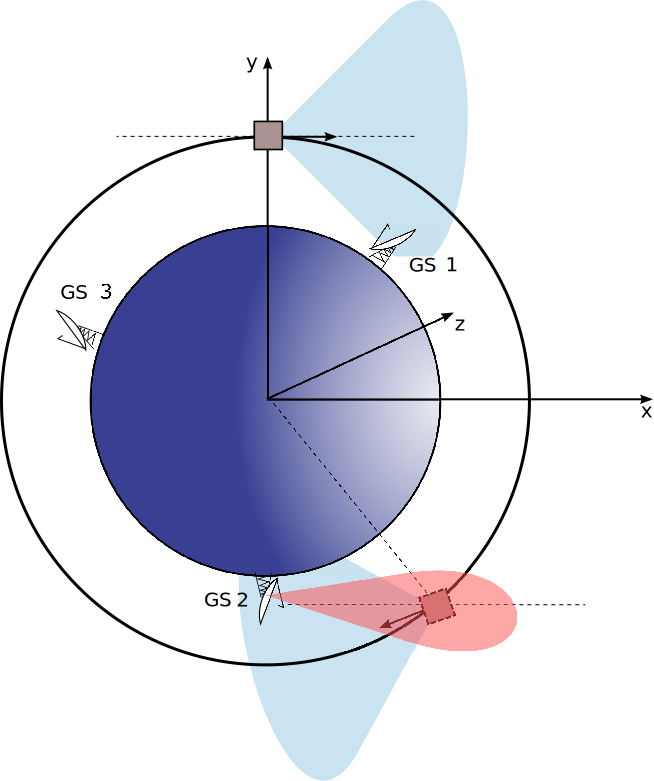
\includegraphics[width=10cm]{images/sms-en.eps}
    \caption{SC in the mission "SMS everywhere"}
    \label{Pic:SMS}
  \end{center}
\end{figure}

Ground stations are located at different points on the earth's surface and are called "0", "1", "2", etc. Each design office receives a unique variant that contains:

\begin{itemize}
\item starting altitude of the orbit;
\item list and names of ground measuring points;
\item message table to send (5 messages in total).
\end{itemize}

The spacecraft must sequentially deliver the maximum number of messages specified in the table. As soon as the device has received a message from the ground station, the countdown of the delivery time begins, which should not exceed the allowable transmission time. The mission is given 6 hours.

The message table has the following format:

\begin{center}
  \begin{tabular}{|p{3.5cm}|p{3.5cm}|p{3.5cm}|p{3.5cm}|}
    \hline
    \textbf{Message Source (ground station)} & \textbf{Message Destination (ground station)} & \textbf{Message Data Size (KB)} & \textbf{Permissible Transmission Delay, s}\\
    \hline
    0 & 3 & 20 & 6212\\
    \hline
    3 & 2 & 26 & 6095\\
    \hline
    \multicolumn{4}{|c|}{...}\\
    \hline
  \end{tabular}
\end{center}

In this mission, you will have to fully calculate and construct the satellite.

\paragraph{Receiving and sending messages}

To receive SC messages, you need to access the high-performance communication subsystem \verb'transmitter'. First of all, you need to enable the subsystem by changing its mode to
\verb'STATE_ON':

\begin{verbatim}
sputnik.transmitter.set_state(STATE_ON)
\end{verbatim}

To receive a message from the ground station on the Earth's surface, use the receive command. This function takes a single parameter~--- the number of the ground station from which the message is expected. This command starts receiving a message. To check if a message has been received, use the \verb'get_progress' function, which returns what percentage of the message has been received (from 0 to 100). After a message is received, the \verb'get_message' function can be used to read the received message.

\begin{verbatim}
sputnik.transmitter.receive(msg_from)
...
if sputnik.transmitter.get_progress(msg_from) == 100.0:
    msg = sputnik.transmitter.get_message(msg_from)
    msg_from = msg.sender
    msg_to = msg.receiver
    data = msg.data
    timeout = msg.timeout
    ...
\end{verbatim}

\textbf{Please note:} between the command to receive a message (\verb'receive') and the fact of receiving the message, some time must necessarily pass, because the message must accumulate in the receive buffer of the high-performance communication subsystem.

Only serial reception of spacecraft messages is possible. In this case, simultaneous reception and forwarding of a message is allowed. In this case, the communication channel is first used to receive information from the spacecraft, and only then, if there is an unused communication band, to send messages.

To subsequently send a message to a ground station on the surface of the Earth, you can use the \verb'send_data' command:

\begin{verbatim}
sputnik.transmitter.send_message(MESSAGE_SMS, data, msg_to, msg_from, timeout)
\end{verbatim}

In this mission, it is fundamentally important to indicate from which ground station the message is sent to, otherwise it may not reach the addressee. \textbf{Beware} of using multi-destination messages in this mission (when \verb'msg_to' is -1). In this case, many ground stations will not receive the messages they expect, and you may not receive mission points at all.

\subsection{Satellite inspection}

The "Satellite Inspection" mission considers the situation of shooting an object that moves in a different orbit around the Earth. It is necessary to photograph the object in the maximum resolution and transmit the resulting image to the ground measuring station (GMS) using high-performance communication.

\paragraph{Initial data}

Each design bureau receives a unique variant that contains: the starting orbit height and the target orbit, as well as the position of the ground station.

During the time allotted for the mission (6 hours), it will be necessary to obtain and transmit to Earth the highest quality image of the inspected object.

\begin{figure}[tbh]
  \begin{center}
    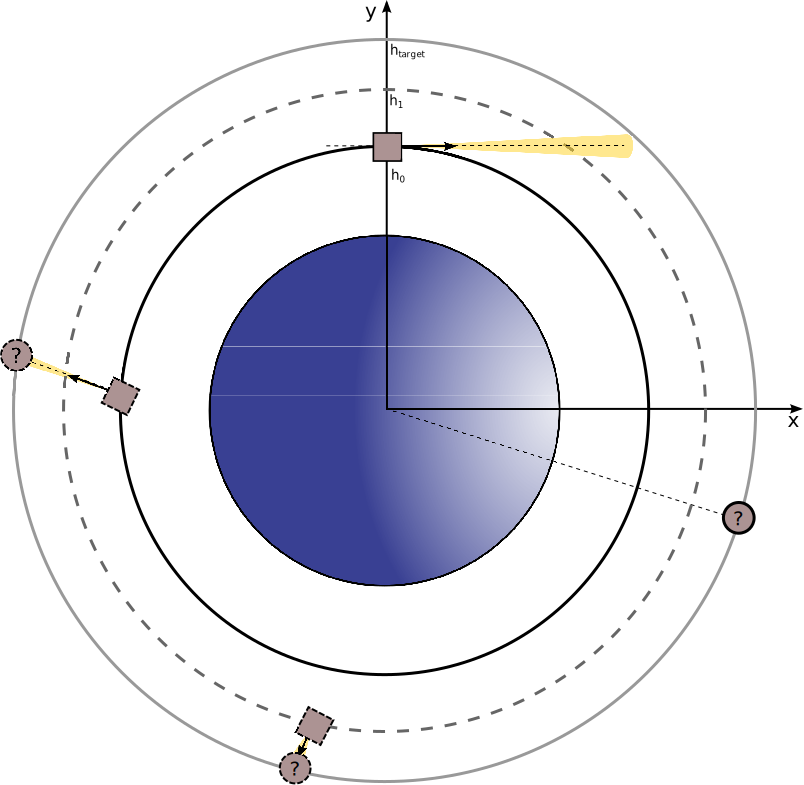
\includegraphics[width=12cm]{images/inspect-en.eps}
    \caption{Spacecraft in the mission "Satellite Inspection"}
    \label{Pic:SMS}
  \end{center}
\end{figure}

The quality of the image (the number of victory points) depends on its resolution (in meters per pixel) and the angle of deviation of the target from the axis of the survey (whether we are pointing exactly at the target). The higher the resolution and the higher the accuracy of the hit, the higher the number of points received per mission. If the subject does not enter the frame at all, such a shot is not counted.

In this mission, you will have to fully calculate and construct the satellite. You will need to select the SC payload~--- optical camera. The details of the physical model associated with the camera are described in the \ref{Sec:Load} section.

One way to reduce the distance to the target on the surface is to transfer the spacecraft to a lower orbit, for which an orbit change subsystem is used, which consists of a propulsion system and fuel tanks. For more information on how to change the spacecraft's orbit, see \ref{Sec:Maneuvre}.

\clearpage
\subsection{Protein crystal in weightlessness}

The Protein Crystal mission is dedicated to scientific experiments in orbit. You will need to grow a protein crystal with the help of special equipment under limited conditions, and then send the device to a given point on the Earth's surface.

\paragraph{Initial data}

Each design bureau receives a unique version that contains: the starting height of the orbit, the orbit in which the experiment should be performed and the point on the Earth's surface where the apparatus should be directed.
\begin{figure}[tbh]
  \begin{center}
    \includegraphics[width=12cm]{images/crystal.eps}
    \caption{Spacecraft in the mission "Protein crystal in weightlessness"}
    \label{Pic:SMS}
  \end{center}
\end{figure}

The success of the mission depends on several parameters. First, it is necessary to transfer the spacecraft to the desired orbit $h_1$ with an accuracy of 1 km for the experiment. Secondly, for the correct operation of scientific equipment, it will be necessary to turn off all subsystems except for the payload and critical ones (onboard computer, EPS and TMS). Thirdly, it will be necessary to maintain a narrow critical temperature range during one rotation around the Earth, which is especially important for the payload. After completing one rotation in a given orbit, the spacecraft can turn back all the systems and go to Earth, where it must land as close as possible to the desired point. We advise you to familiarize yourself with the features of the physical model of the spacecraft's movement (see the \ref{Sec:Ballistics} section) and the method of changing the spacecraft's orbit (see the \ref{Sec:Maneuvre} section).

The container is controlled using two commands \verb'start_experiment' and \verb'stop_experiment' without parameters.

In this mission, you will have to fully calculate and construct the satellite. You will need to select the SC payload~--- the container for the crystal.

\paragraph{Landing on Earth}

In this mission you will have to land on Earth. To land on Earth, it is necessary to make a braking impulse, after which the spacecraft will begin to descend to a certain point on the surface. In this case, it is necessary to prevent the destruction of the spacecraft in the atmosphere.

It is believed that in this mission the device has a slightly different design: a second, heat-resistant spherical body is hidden under the cubic body. When landing, it is necessary to take into account the Earth's atmosphere, the properties of which can be found in GOST 4401-81 “Standard atmosphere. Parameters ”(the table is easy to find on Wikipedia). When descending in the atmosphere, the spacecraft is affected by the aerodynamic drag force directed against the velocity vector and calculated by the formula \ref{Eq:stokes}:

$$
  F_{\text{А}} = C_\xi \frac{\rho V_{\text{SC}}^2}{2} S_{\text{SC}},
  $$

where $C_\xi$~-- is the aerodynamic drag coefficient of the spacecraft; $\rho$~--– atmospheric density at the current spacecraft flight altitude, $\text{kg}/\text{m}^3$; $V_{\text{SC}}$~--– current
spacecraft flight speed, m/s; $S_{\text{SC}}$~--- SC cross-sectional area, $\text{m}^2$. The aerodynamic drag force $F_{\text{А}}$ is directed opposite to the spacecraft velocity vector, see figure \ref{Pic:Stokes}.

Thus, when passing through the dense layers of the atmosphere, the spacecraft will experience increased overloads. The design of the spacecraft has a tensile spacecraft, the maximum allowable overload is $10g$ (98.1 m/s). Exceeding this limit leads to the destruction of the device.

To enter the atmosphere, you need to execute the \verb'container.drop()' function. After that, the container fires back and makes a ballistic fall to the Earth, and the device itself is destroyed in the dense layers of the atmosphere. The container has the following options:

\begin{itemize}
   \item mass is equal to the initial mass of the container;
   \item the container is assumed to be spherical, so knowing its volume, you can calculate its cross-sectional area;
   \item the characteristic area of the spherical spacecraft $C_{\xi}$ is equal to 0.47.
\end{itemize}

A parachute can be used to soften the landing. The parachute opening is programmed: before dropping the container, you must set the height in meters at which the parachute should open:

\begin{verbatim}
container.set_parachute_height(h)
\end{verbatim}

The parachute has the following parameters:

\begin{itemize}
\item parachute area depends on container type (for a small container it is 3 $\text{m}^2$, for a large container~--— 20 $\text{m}^2$);
\item the characteristic area of the parachute $C_{\xi}$ is equal to 0.9.
\end{itemize}

The force of aerodynamic resistance from the parachute is added to the force from the friction of the container itself.
Landing is considered successful if the speed of the spacecraft has decreased to \textbf{20 m/s}.

When calculating orbits and landing on Earth, we recommend using the Ballistic Calculator (see \ref{Sec:Calculator}).

\clearpage
\subsection{Communication satellite <<Molniya>>}

The Molniya Communications Satellite mission simulates a situation in which it is necessary, having a limited resource in terms of fuel and satellite parameters, to organize several sessions of long-term radio communication with a ground measuring point. It turns out that the usual circular orbits are not suitable for solving the problem and you need to figure out how to replace them.

\begin{figure}[tbh]
  \begin{center}
    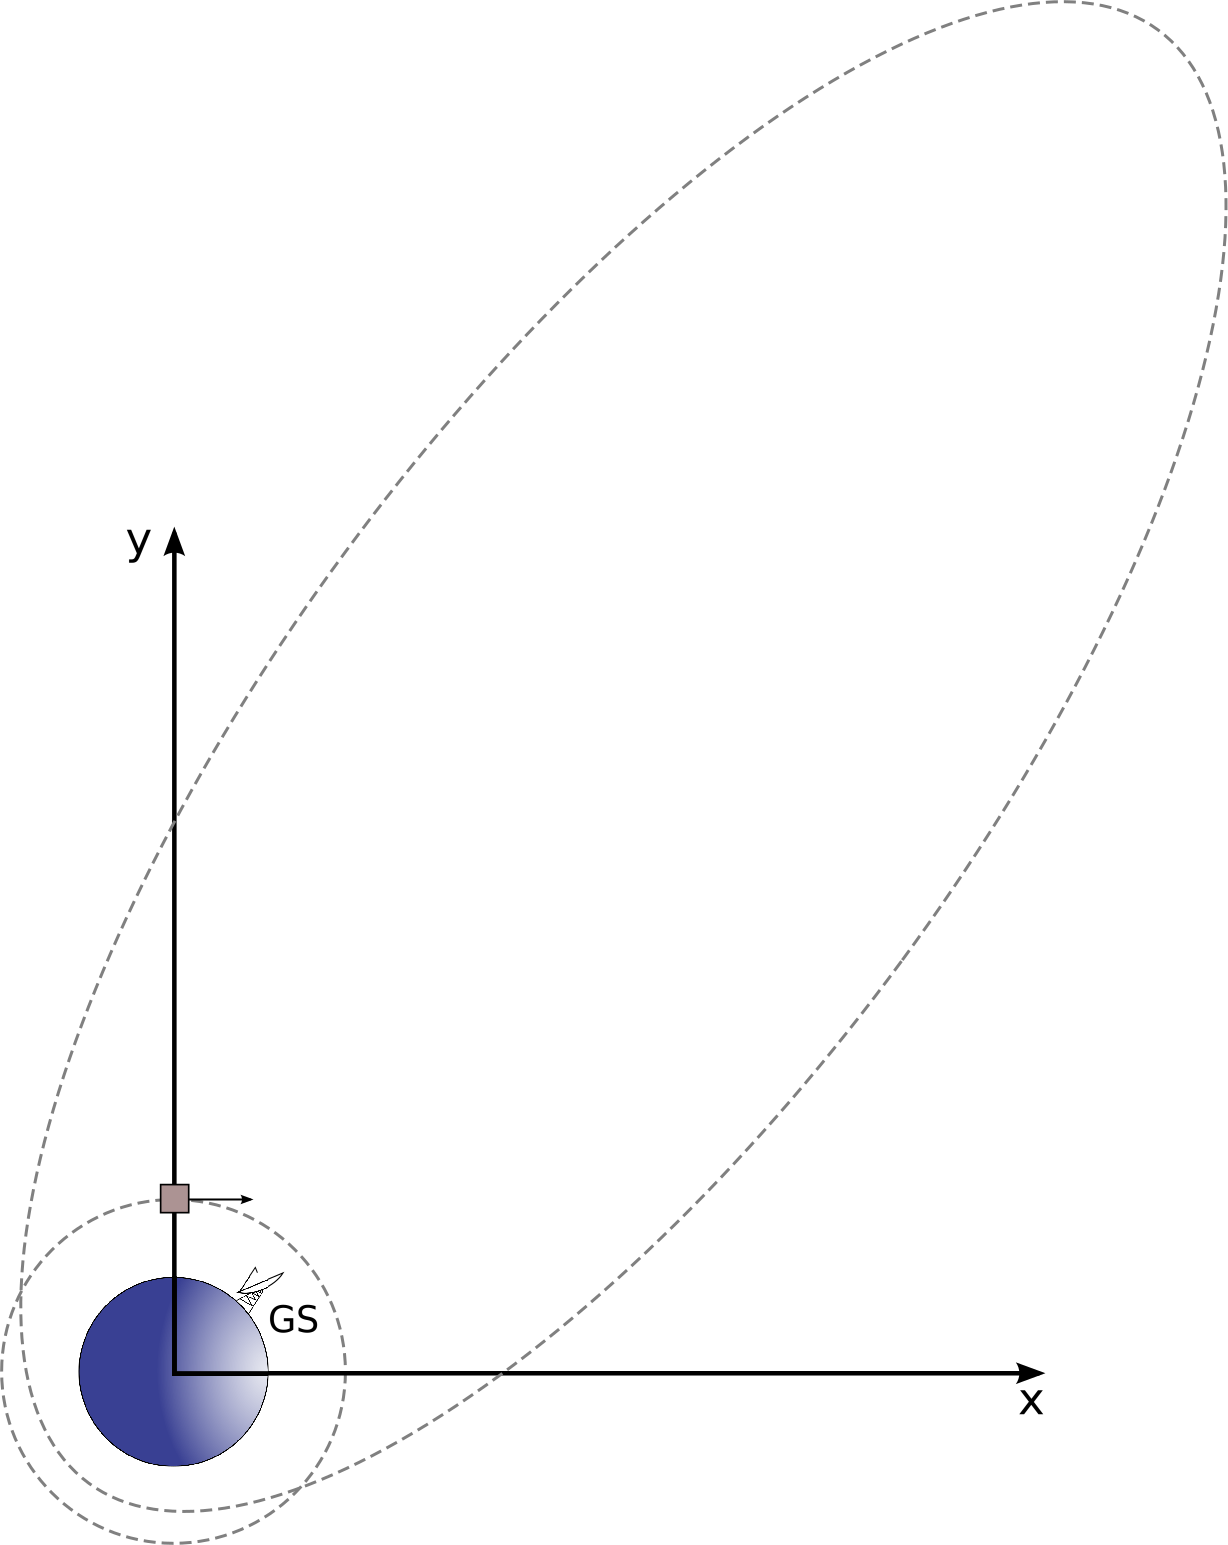
\includegraphics[width=10cm]{images/molniya-en.eps}
    \caption{The ratio of the circular orbit and the "Molniya" orbit}
    \label{Pic:Molniya}
  \end{center}
\end{figure}

\paragraph{Initial data}

Your spacecraft is in a circular low orbit. To complete the mission, you need to conduct two communication sessions with a ground station lasting at least 8 hours with a channel bandwidth of at least \textbf{1 Mb/s}. A communication session is such a state of the satellite when it has a high-speed transmitter continuously turned on, and the ground station is in the transmitter coverage area. In order to have such a long communication session, during the course of the mission, you will have to move the satellite into a suitable elliptical orbit. Please note that this mission simulates the rotation of the Earth along with the ground stations located on it. The Earth completes one rotation in 23 hours and 56 minutes.

The simplest solution for such a task would be a geostationary satellite located above the ground station, however, in our case, the satellite does not have enough fuel to go from the low orbit in which it is at the start of the task, immediately to the geostationary orbit. A possible solution to this problem is the Molniya orbit, named after the Soviet Molniya communications satellites (see figure \ref{Pic:Molniya}). This orbit is a highly elongated elliptical orbit with an apogee of about 40,000 kilometers and a perigee of about 600 km, with the Earth at one of the foci of this orbit. Since the total energy of the mechanical energy of the apparatus is conserved, as it moves away from the Earth (i.e., approaches the apogee), the velocity of the apparatus will decrease, and at the maximum distance, the apparatus in such an orbit will be able to stay in the observation zone of the ground station for a long time.

\paragraph{Elliptical orbit}

To solve the problem, you will need to determine the parameters of the orbit in which the satellite should be, write a program for transferring to this orbit (training missions will help you with this), and orient the satellite to the ground station for successful transmission.

The choice of orbit is determined by the condition that your craft sees the ground station continuously for \textbf{8 hours} and, at the same time, passes through such an orbit at least twice. Almost all circular orbits that are available in terms of fuel supply for your vehicle to go are too low and the vehicle will lose ground station significantly faster than 8 hours. The solution is elliptical orbits, the exact parameters of one of which must be selected.

\begin{figure}[tbh]
  \begin{center}
    \includegraphics[width=10cm]{images/ellipse.eps}
    \caption{Elliptical orbit parameters}
    \label{Pic:Ellipse}
  \end{center}
\end{figure}

An apparatus (artificial Earth satellite) moving in an elliptical orbit (see figure \ref{Pic:Ellipse}) revolves around the Earth located at one of the foci of the ellipse (point <<З>>). It will fly closest to the Earth at the perigee (point <<P>>), and farthest at the apogee (point <<A>>). An ellipse is defined by its semi-major axis (<<AO>>) and eccentricity $e$, which is calculated by the formula:

\begin{eqnarray}
  e = \sqrt{1 - \frac{b^2}{a^2}},
\end{eqnarray}

where $a$~--- the major semi-axis of the ellipse and $b$~--- the minor semi-axis.

Using Kepler's laws, we can obtain the following relationship for the distance to the Earth and the spacecraft's speed at different points of the orbit (depending on the angle $\theta$):

\begin{eqnarray}
  r(\theta) = \frac{a (2 - e^2)}{1 + e \cdot \cos\theta},\\
  V(\theta) = V_I \sqrt{\frac{2 R}{r(\theta)} - frac{R}{a}},
\end{eqnarray}

where $V_I = \sqrt{\frac{G M}{R}}$~--- the first escape velocity of the Earth, equal to 7.91 km/h.

The orbital period of a satellite in an elliptical orbit can be calculated as:

\begin{eqnarray}
  T = \frac{2 \pi R}{V_I} \cdot \left( \frac{a}{R} \right)^{\frac{3}{2}}
\end{eqnarray}

\paragraph{Transfer to elliptical orbit}

The new elliptical orbit of the satellite will be determined by the point at which the satellite was at the time the engine was turned on, and its final speed.

To transfer to an elliptical orbit, you can use both a two-pulse transfer, similar to that used in the <<Orbit maneuver>> training mission (section \ref{Sec:Maneuvre}), and a single-pulse transfer, which is much easier to calculate. For a stationary Earth, such a transfer would have to start at a point diametrically opposite to the ground station, however, in our problem, the Earth rotates, and you will have to determine the point at which you actually need to make the transfer yourself. The speed increment can be calculated using the formula given in the Orbit Maneuver mission description for the first transfer:

\begin{eqnarray}
  \Delta V = V_I \left(\sqrt{\frac{2 R_2}{R_1 + R_2}} - 1 \right),
\end{eqnarray}

where $R_1$~--- the reference orbit where your spacecraft is initially located, and $R_2$~--- the distance from the center of the Earth to the apogee of your planned orbit. Since you don't need to re-enter the circular orbit, the second transition is not needed. Further considerations are similar to those given in the description of the Orbit Maneuver mission.

\paragraph{Transmitter}

You must select the devices installed on your satellite. In our case, the transmitter will be the main such device.

You need to transmit a certain set of data to Earth, providing a channel with a bandwidth of \textbf{1 Mb/s} for \textbf{8} hours of continuous transmission. A communication session is such a state of the satellite when it has a high-speed transmitter continuously turned on, and the ground station is in the transmitter coverage area. This requires a transmitter having certain properties. The onboard transmitter antenna is fixed on the surface of the spacecraft and is characterized by a radiation pattern, and different transmitters have different radiation patterns and transmitter channel bandwidth parameters.

The description of the model and the calculation technique are described in the section \ref{Sec:Radio}.

\paragraph{Heat and energy balance}

After choosing the type of transmitter, it is necessary to determine the algorithm for its activation, which in turn depends on the orientation of the spacecraft to the ground station. The easiest way is to orient your spacecraft to the center of the Earth. This may be enough to solve it, but if you manage to orient the device exactly to the ground station, you will get extra points.

After the main parameters of the orbit and spacecraft are calculated and set, it is necessary to check the energy and heat balance of the spacecraft in the same way as it was done in the Earth Communications mission (section \ref{Sec:Test2}). It must be taken into account that for a sufficiently long time, due to the elongated orbit, the device will be illuminated by the Sun and may overheat.

\clearpage
\subsection{Missile warning system}

In today's world filled with nuclear weapons, satellites perform an extremely important function of preventing missile launches. During acceleration, a ballistic missile releases a large amount of energy and is clearly visible in the infrared range. A satellite in orbit, using an infrared camera, can easily identify the launch site of a rocket, and this makes interception possible.

\paragraph{Initial data}

Your spacecraft is in geostationary orbit. His area of responsibility~--- sector of the earth's surface \textbf{±45 degrees} from the point of standing. Ballistic missiles will be launched from this region during the mission, which must be detected and intercepted. On the active leg of the flight, the rocket torch is clearly visible in the IR range. The active phase lasts \textbf{180 seconds}, during which time the misile reaches an altitude of about \textbf{160 km}.

\begin{figure}[tbh]
  \begin{center}
    \includegraphics[width=12cm]{images/early-warning.eps}
    \caption{Spacecraft in the mission "Missile attack warning system"}
    \label{Pic:EWarning}
  \end{center}
\end{figure}

Your spacecraft must make round-the-clock surveys of the Earth with the help of an IR telescope and promptly transmit the received data to the Earth. To successfully intercept a missile, a snapshot with its image must be transmitted to Earth no later than \textbf{180 seconds} after launch. To obtain a sufficiently complete coverage of the surface, it is recommended to shoot with an angular velocity of rotation of the spacecraft no more than \textbf{1°/s}.

Please note that this mission simulates the rotation of the Earth along with the ground stations located on it. The Earth completes one rotation in 23 hours and 56 minutes.

\paragraph{Observation}

The spacecraft is not equipped with the means of processing the received information, therefore, after each image, it must be transmitted to Earth. Taking into account the time it takes for the rocket to take off, once every 180 seconds your spacecraft must scan each section of the zone accountable to it and transmit each received image to the ground station. In this task, this means that it is necessary to send the received image to the ground station immediately after shooting one frame.

\paragraph{Spacecraft Orientation}

Your spacecraft is in geostationary orbit. This means that it is always above one point on the equator, the longitude of which is called the standing point. The height of such an orbit is \textbf{35794 km}. In order for the satellite camera to always look at this point, after stabilization, the spacecraft must be oriented to it, and then rotated with an angular velocity that coincides with the angular velocity of the spacecraft around the Earth. However, to successfully detect missiles, you need to look not only at this point, but also at all points on the Earth's surface, the longitude of which differs from the standing point by \textbf{45 degrees}, both up and down. In the picture \ref{Pic:EWarning} this area is marked in red.

This means that an additional periodic rotation of the spacecraft is superimposed on the constant rotation, the parameters of which you need to choose yourself.

In this mission, the experience of the training mission "Look at the Earth" will help you, except that the angular velocity of the spacecraft will not be constant. In this case, the angular velocity of the spacecraft cannot be changed directly. You can only control the momentum of the flywheel. The obvious solution~--- set the angular momentum as a function of time ~--- theoretically it can be good, but in real problems, in particular, in this one, errors will accumulate too quickly. The correct solution would be to implement a feedback system. For example, you can specify the dependence of the flywheel momentum not on time, but on the angle and angular velocity.

\paragraph{Infrared telescope}

To take pictures, your spacecraft must be equipped with an IR telescope. An IR telescope is one of the "camera" type objects. A detailed physical model of the camera is presented in the \ref{Sec:Load} section.

The camera is controlled through special commands in the flight program. It is possible to take a single shot or shoot a stream of frames. The image taken by the camera must be completely transmitted to Earth via a high-performance communication channel.

Another important parameter of the camera is the amount of RAM of the computer system. When the camera is turned on, the data stream begins to continuously enter the memory of the computer system. The picture is sent to the radio channel after the camera is turned off. If the RAM of the camera's computing system becomes full, the existing image is discarded. So you can lose a good shot.

\paragraph{Camera control}

The camera is controlled by calling special methods of the payload subsystem. To take pictures, the camera must be turned on (be in \verb'STATE_ON' mode). You can use the following methods to take a snapshot:

\begin{itemize}
\item \verb'camera.take_photo()'~--— The IR telescope takes a snapshot (with a duration of \textbf{0.01 s}), the method returns the number of the memory block in which the snapshot is stored;
\item \verb'camera.start_shooting()'~--— IR telescope starts continuous shooting;
\item \verb'camera.stop_shooting()'~--- stop continuous shooting, the method returns the number of the memory block in which the captured strip of the surface is stored.
\end{itemize}

Thus, you have two ways of shooting~--- single-frame and continuous. In any case, the output should be a block of memory in which the snapshot required by the conditions of the task is stored. It must be transmitted to Earth through a special call to the high-performance communication subsystem:

\begin{verbatim}
slot = sputnik.take_photo()
sputnik.transmitter.send_photo(slot)
\end{verbatim}

\paragraph{Transmitter}

You need to transmit the survey results to Earth. This requires a transmitter with certain properties. The onboard antenna of the transmitter is fixed on the surface of the spacecraft and is characterized by a radiation pattern, and different transmitters have different radiation patterns and channel throughput parameters. For more information about working with the transmitter, see the \ref{Sec:Radio} section.

\paragraph{Heat and energy balance}

After the main parameters of the orbit and spacecraft are calculated and set, it is necessary to check the energy and heat balance of the spacecraft in the same way as it was done in the Earth Communications mission (section \ref{Sec:Test2}). Please note that during the passage of the mission, the device will heat up rather slowly, and then quickly cool down. It is necessary to choose the ratio of reflective surfaces and radiators in such a way that all devices can withstand the temperature regime.

\clearpage
\section{Competitions}

For the successful solution of the mission, participants receive victory points. The mission parameters are described in the \verb'missions.xml' file and include the victory conditions along with the corresponding points for the participating team. The victory conditions can be divided into two types~--- the speed of solving the problem and the fulfillment of the special parameters of each of the missions.

In addition, a set of start launches can be specified for each mission (for example, \textbf{10}). In this case, for each run after the \textbf{10}th one, a penalty can be added, for example, \textbf{150 points} per run, and so on up to \textbf{20} additional runs (total up to \textbf{-3000 points} ).

The final points of the teams are summed up and form the leader board of the teams.
The following are the suggested levels of victory points for each of the missions:

\begin{center}
\begin{longtable}{ |p{5cm}|p{8cm}|c|}
  \hline
  \textbf{Status} & \textbf{Explanation} & \textbf{Points}\\
  \hline
  \endhead
  \multicolumn{3}{|c|}{\textbf{Looking at the Earth}}\\
  \hline
  First in Orbit & Complete the mission first & 60\\
  \hline
  Second in Orbit & Complete mission second & 50\\
   \hline
   Third in orbit & Complete the mission as third & 40\\
   \hline
   On the first try & Complete the mission on the first try & 50\\
   \hline
   On the second try & Complete the mission on the second try & 30\\
   \hline
   Mission accomplished & Complete the mission on the third or more attempts & 10\\
   \hline
   Completed in one orbit & The mission was completed in just one orbit around the Earth & 50\\
  \hline
  \multicolumn{3}{|c|}{\textbf{Communication with the Earth}}\\
  \hline
  First in Orbit & Complete the mission first & 200\\
  \hline
 Second in Orbit & Complete mission second & 175\\
  \hline
  Third in orbit & Complete the mission as third & 150\\
  \hline
  On the first try & Complete the mission on the first try & 120\\
  \hline
  On the second/third try & Complete the mission on the second or third try & 100\\
  \hline
  Mission accomplished & Complete the mission on the fourth or more attempts & 80\\
  \hline
 Completed in one orbit & The mission was completed in just one orbit around the Earth & 200\\
  \hline
  \multicolumn{3}{|c|}{\textbf{Orbit maneuver}}\\
  \hline
  First in Orbit & Complete the mission first & 300\\
   \hline
   Second in Orbit & Complete mission second & 280\\
   \hline
   Third in orbit & Complete the mission as third & 250\\
   \hline
   On the first try & Complete the mission on the first try & 1000\\
   \hline
   From 2-5 attempts & Complete mission from 2-5 attempts & 400\\
   \hline
   Mission Accomplished & Complete mission with 6th or more & 100\\
   \hline
   Accurate calculation & The difference between the spacecraft orbit and the target orbit is no more than 1000 m & 1000\\
   \hline
  \multicolumn{3}{|c|}{\textbf{Earth remote sensing}}\\
  \hline
First in Orbit & Complete the mission first & 1200\\
   \hline
   Second in Orbit & Complete mission second & 1000\\
   \hline
   Third in orbit & Complete the mission as third & 800\\
   \hline
   Perfect Calculation & Complete the mission on the first try & 3000\\
   \hline
   High reliability & Complete the mission on the second to fifth attempt & 2000\\
   \hline
   Mission accomplished & Complete the mission on 6th or more attempts & 1000\\
   \hline
   High image resolution & Image resolution better than 10m per pixel & 5000\\
   \hline
   Precise hit & Angle of deviation from the target $\theta$ does not exceed 0.01° & 3000\\
   \hline
   Vertical survey & Angle of deviation from normal $\beta$ does not exceed 0.01° & 2000\\
   \hline
   \multicolumn{3}{|c|}{\textbf{SMS everywhere}}\\
   \hline
First in Orbit & Complete the mission first & 1500\\
   \hline
   Second in Orbit & Complete mission second & 1200\\
   \hline
   Third in orbit & Complete the mission as third & 1000\\
   \hline
   Perfect Calculation & Complete the mission on the first try & 3000\\
   \hline
   Accurate calculation & Complete the mission on the second to fifth attempt & 2000\\
   \hline
   Mission accomplished & Complete the mission on 6th or more attempts & 1000\\
   \hline
   High reliability & Accurately sent at least 5 messages & 5000\\
   \hline
   \multicolumn{3}{|c|}{\textbf{Satellite Inspection}}\\
   \hline
   First in Orbit & Complete Mission First & 2000\\
   \hline
   Second in Orbit & Complete mission second & 1800\\
   \hline
   Third in orbit & Complete the mission as third & 1600\\
   \hline
   Perfect Calculation & Complete the mission on the first try & 6000\\
   \hline
   High reliability & Complete the mission on the second to fifth attempt & 4000\\
   \hline
   Mission Accomplished & Complete the mission on 6th or more attempts & 2000\\
   \hline
   High image resolution & Resolution of the examined object is not worse than 1 m per pixel & 10000\\
   \hline
   Crept up to the target & Distance to the investigated object is no more than 1000 m & 10000\\
  \hline
\multicolumn{3}{|c|}{\textbf{Protein crystal in weightlessness}}\\
   \hline
   First in Orbit & Complete the mission first & 2400\\
   \hline
   Second in Orbit & Complete mission second & 2200\\
   \hline
   Third in Orbit & Complete the mission as third & 2000\\
   \hline
   Perfect Calculation & Complete the mission on the first try & 8000\\
   \hline
   High reliability & Complete the mission on the second to fifth attempt & 6000\\
   \hline
   Mission accomplished & Complete mission on 6th or more attempts & 3000\\
   \hline
   Stable experimental conditions & Temperature deviation during the experiment is not
   exceeds 1° & 10000\\
   \hline
   Accurate landing & Landing point deviation less than 1° & 10000\\
   \hline
    \multicolumn{3}{|c|}{\textbf{Communication satellite «Molniya»}}\\
   \hline
   First in Orbit & Complete Mission First & 2000\\
   \hline
   Second in Orbit & Complete mission second & 1800\\
   \hline
   Third in orbit & Complete the mission as third & 1600\\
   \hline
   Perfect Calculation & Complete the mission on the first try & 6000\\
   \hline
   High reliability & Complete the mission on the second to fifth attempt & 4000\\
   \hline
   Mission Accomplished & Complete the mission on 6th or more attempts & 2000\\
   \hline
   Lightning Deployment & Have at least 3 comms during the mission & 5000\\
   \hline
   Not a single break & The duration of each session is at least 10 hours & 10000\\
   \hline
   \multicolumn{3}{|c|}{\textbf{Missile Warning System}}\\
   \hline
   First in Orbit & Complete the mission first & 2400\\
   \hline
   Second in Orbit & Complete mission second & 2200\\
   \hline
   Third in Orbit & Complete the mission as third & 2000\\
   \hline
   Perfect Calculation & Complete the mission on the first try & 8000\\
   \hline
   High reliability & Complete the mission on the second - fifth attempt & 6000\\
   \hline
   Mission accomplished & Complete mission on 6th or more attempts & 3000\\
   \hline
   You shall not pass! & All missiles were intercepted & 10000\\
  \hline
\end{longtable}
\end{center}

\section*{List of abbreviations}
\addcontentsline{toc}{section}{List of abbreviations}

\begin{description}
\item[OCC] on-board central computer;
\item[SC] spacecraft;
\item[GS] ground station;
\item[TMS] thermal management subsystem;
\item[PV] photovoltaic cells.
\end{description}

\begin{thebibliography}{2}
\addcontentsline{toc}{section}{References}
\bibitem{SMAD} J.~R. Wertz, D.~F. Everett, J.~J. Puschell. Space mission
engineering: the new SMAD, 2011.
\bibitem{MECHANICS} Open online course <<
Toggle the table of contents
Celestial mechanics>>~---
  \url{https://www.lektorium.tv/skymechanics}
\bibitem{SHAENKO} A. Shaenko. Open online course <<Designing space technology>> ~---
  \url{https://stepik.org/course/2119/}
\end{thebibliography}

\section*{Appendix 1. Reference book of available subsystems}
\label{Sec:Subsystems}
\addcontentsline{toc}{section}{Appendix 1. Reference book of available subsystems}

The list of variants of subsystems of the device available for designing is presented in the table:

\begin{center}
  \begin{longtable}{|p{2.5cm}|p{2cm}|c|c|c|p{3.8 cm}|}
  \hline
  \textbf{Name} &
  \begin{tabular}{c}
    \textbf{Weight,}\\
    \textbf{kg}
  \end{tabular} &
  \begin{tabular}{c}
    \textbf{Volume,}\\
    \textbf{l}
  \end{tabular} &
  \begin{tabular}{c}
    \textbf{Temp.}\\
    \textbf{mode}\\
    \textbf{min./}\\
    \textbf{max.,}\\
    \textbf{°С}
  \end{tabular} &
  \begin{tabular}{c}
    \textbf{Power}\\
    \textbf{and heat,}\\
    \textbf{W}
  \end{tabular} &
  \textbf{Add. options}\\
  \hline
  \endhead
  \multicolumn{6}{|c|}{\textbf{Hull}}\\
  \hline
  Hull for CubeSat-1U & 0,3 & 1,1 & -100 / 100 & 0 &
  \begin{tabular}{p{3.5cm}}
  Spacecraft side: $\sqrt[3]{1,1\cdot 10^{-3}} = 0,1032280$ m
  \end{tabular} \\
  \hline
  Hull for CubeSat-3U & 1 & 3,4 & -100 / 100 & 0 &
  \begin{tabular}{p{3.5cm}}
 Spacecraft side: $\sqrt[3]{3,4\cdot 10^{-3}} = 0,1503695$ m
  \end{tabular} \\
  \hline
  Hull for CubeSat-6U & 2 & 6,8 & -100 / 100 & 0 &
  \begin{tabular}{p{3.5cm}}
 Spacecraft side: $\sqrt[3]{6,8\cdot 10^{-3}} = 0,1894536$ m
  \end{tabular} \\
  \hline
  Hull for microsatellite & 10 & 125 & -100 / 100 & 0 &
  \begin{tabular}{p{3.5cm}}
 Spacecraft side: $\sqrt[3]{125\cdot 10^{-3}} = 0,5$ m
  \end{tabular} \\
  \hline
  Hull for minisatellite & 25 & 512 & -100 / 100 & 0 &
  \begin{tabular}{p{3.5cm}}
   Spacecraft side: $\sqrt[3]{512\cdot 10^{-3}} = 0,8$ m
  \end{tabular} \\
  \hline
  \multicolumn{6}{|c|}{\textbf{On-board central computers}}\\
  \hline
  On-board central computer-1 & 0,4 & 0,15 & -40 / 80 & 1 &
  \begin{tabular}{p{3.5cm}}
  Processor frequency: 60 MHz\\
  Memory capacity: 16 MB
  \end{tabular} \\
  \hline
  On-board central computer-2 & 1,5 & 0,8 & -40 / 80 & 3,5 &
  \begin{tabular}{p{3.5cm}}
  Processor frequency: 150 MHz\\
  Memory capacity: 64 MB
  \end{tabular} \\
  \hline
  On-board central computer-3 & 6,0 & 5,5 & -40 / 50 & 23 &
  \begin{tabular}{p{3.5cm}}
  Processor frequency: 228 MHz\\
  Memory capacity: 512 MB
  \end{tabular} \\
  \hline
  \multicolumn{6}{|c|}{\textbf{Navigation system}}\\
  \hline
  Navigator-1 & 0,4 & 0,15 & -40 / 60 & 0,5 &
  \begin{tabular}{p{3.5cm}}
  Processor frequency: 15 MHz\\
  Memory capacity: 0,5 MB
  \end{tabular} \\
  \hline
  Navigator-2 & 0,3 & 0,6 & -40 / 60 & 2 &
  \begin{tabular}{p{3.5cm}}
  Processor frequency: 60 MHz\\
  Memory capacity: 0,5 MB
  \end{tabular} \\
  \hline
  \multicolumn{6}{|c|}{\textbf{Attitude and stabilization control system}}\\
  \hline
  Orientation system with low control torque & 0,2 & 0,2 & -20 / 50 & 1 &
  \begin{tabular}{p{3.5cm}}
  Processor frequency: 15 MHz\\
  Maximum moment: 0,000023 $\text{Н} \cdot \text{м}$\\
  Memory capacity: 0,5 MB\\
  Type of orientation device: flywheel
  \end{tabular} \\
  \hline
  Orientation system with medium control torque & 2,0 & 1,5 & -20 / 60 & 5 &
  \begin{tabular}{p{3.5cm}}
  Processor frequency: 40 MHz\\
  Maximum moment: 0,0026 Н м\\
  Memory capacity: 16,5 MB\\
  Type of orientation device: flywheel
  \end{tabular} \\
  \hline
  High torque orientation system & 6,6 & 8,7 & -20 / 50 & 15 &
  \begin{tabular}{p{3.5cm}}
  Processor frequency: 84 MHz\\
  Maximum moment: 0,0165 $\text{Н} \cdot \text{м}$\\
  Memory capacity: 8 MB\\
  Type of orientation device: flywheel
  \end{tabular} \\
  \hline
  Orientation system with very high control torque & 45 & 60 & -20 / 50 & 50 &
  \begin{tabular}{p{3.5cm}}
  Processor frequency: 80 MHz\\
  Maximum moment: 0,25 $\text{Н} \cdot \text{м}$\\
  Memory capacity: 8 MB\\
  Type of orientation device: flywheel
  \end{tabular} \\
  \hline
  \multicolumn{6}{|c|}{\textbf{Power supply system}}\\
  \hline
  Small battery power system & 0.5 & 0.3 & -10 / 40 & 0.2 &
   \begin{tabular}{p{3.5cm}}
   Absorption coefficient: 0.95 \\
   Battery capacity: 41.8Wh\\
   Maximum charge current: 4A\\
   Maximum discharge current: 4A\\
   Radiator emissivity: 0.4 \\
   Efficiency of photovoltaic cells: 29.8%
  \end{tabular} \\
  \hline
  Medium battery power system & 1,5 & 1,0 & 0 / 40 & 2 &
  \begin{tabular}{p{3.5cm}}
  Absorption coefficient: 0,95 \\
  Battery capacity: 129,6 Wh\\
  Maximum charge current: 10 А\\
  Maximum discharge current 10 А\\
  Radiator emissivity: 0,4 \\
  Efficiency of photovoltaic cells: 28\%
  \end{tabular} \\
  \hline
  Large battery power system & 3,0 & 2,0 & 0 / 40 & 3,5 &
  \begin{tabular}{p{3.5cm}}
  Absorption coefficient: 0,95 \\
  Battery capacity: 259,2 Wh\\
  Maximum charge current: 20 А\\
  Maximum discharge current 20 А\\
  Memory capacity: 2 МБ\\
  Radiator emissivity: 0,4 \\
  Efficiency of photovoltaic cells: 28\%
  \end{tabular} \\
  \hline
  Very large battery power system & 12,0 & 8,0 & 0 / 40 & 5 &
  \begin{tabular}{p{3.5cm}}
  Absorption coefficient: 0,95 \\
  Battery capacity: 1036,8 Wh\\
  Maximum charge current: 40 А\\
  Maximum discharge current 40 А\\
  Radiator emissivity: 0,4 \\
  Efficiency of photovoltaic cells: 28\%
  \end{tabular} \\
  \hline
  \multicolumn{6}{|c|}{\textbf{Telemetry system}}\\
  \hline
  Telemetry with directional antenna & 0.3 & 0.2 & -40 / 80 & 1 &
   \begin{tabular}{p{3.5cm}}
   On-board antenna gain: 2 \\
   Processor frequency: 30MHz\\
   Frequency: 435MHz\\
   Ground antenna gain: 16 \\
   Memory capacity: 16 MB\\
   Antenna Angle: 180°\\
   Emitter power: 0.5W
  \end{tabular} \\
  \hline
  Telemetry with omni directional antenna & 0,6 & 0,4 & -40 / 80 & 2 &
  \begin{tabular}{p{3.5cm}}
   Onboard antenna gain: 1 \\
   Processor frequency: 15MHz\\
   Frequency: 435MHz\\
   Ground antenna gain: 16 \\
   Memory capacity: 8 MB\\
   Antenna Angle: 360°\\
   Emitter power: 1W
   \end{tabular} \\
   \hline
   \multicolumn{6}{|c|}{\textbf{Thermal Management System}}\\
  \hline
 Thermal Management System with Small Heater & 0,3 & 0,1 & -40 / 80 & 0,1 / 4,1 &
  \begin{tabular}{p{3.5cm}}
  Absorption coefficient: 0,2 \\
  Processor frequency: 15 MHz\\
  Memory capacity: 0,5 MB\\
  Radiator emissivity: 1
  \end{tabular} \\
  \hline
  Thermal management system with middle heater & 1,5 & 0,5 & -40 / 80 & 0,2 / 20,2 &
  \begin{tabular}{p{3.5cm}}
  Absorption coefficient: 0,2 \\
  Processor frequency: 15 MHz\\
  Memory capacity: 0,5 MB\\
  Radiator emissivity: 1
  \end{tabular} \\
  \hline
  Thermal management system with large heater & 3 & 1 & -40 / 80 & 0,3 / 40,3 &
  \begin{tabular}{p{3.5cm}}
  Absorption coefficient: 0,2 \\
  Processor frequency: 15 MHz\\
  Memory capacity: 0,5 MB\\
  Radiator emissivity: 1
  \end{tabular} \\
  \hline
  Thermal management system with extra large heater & 7,5 & 2,5 & -40 / 80 & 0,5 / 100,5 &
  \begin{tabular}{p{3.5cm}}
  Absorption coefficient: 0,2 \\
  Processor frequency: 15 MHz\\
  Memory capacity: 0,5 MB\\
  Radiator emissivity: 1
  \end{tabular} \\
  \hline
  \multicolumn{6}{|c|}{\textbf{Orbit Correction System}}\\
   \hline
   Low Thrust Small Tank Engine & 2 & 3 & -100 / 100 & 2 &
   \begin{tabular}{p{3.5cm}}
   Fuel tank volume: 1 l\\
   Specific impulse of the propulsion system: 2790 m/s\\
   Maximum mass flow: 0.009 kg/s\\
   \end{tabular} \\
   \hline
   Medium tank low thrust engine & 5 & 14 & -100 / 100 & 2 &
   \begin{tabular}{p{3.5cm}}
   Fuel tank volume: 10 l\\
   Specific impulse of the propulsion system: 2790 m/s\\
   Maximum mass flow: 0.009 kg/s\\
   \end{tabular} \\
   \hline
   Medium Thrust Medium Tank Engine & 8 & 18 & -100 / 100 & 5 &
   \begin{tabular}{p{3.5cm}}
   Fuel tank volume: 10 l\\
   Specific impulse of the propulsion system: 2705 m/s\\
   Maximum mass flow: 0.037 kg/s\\
   \end{tabular} \\
   \hline
   Medium thrust engine with large tank & 16 & 65 & -100 / 100 & 5 &
   \begin{tabular}{p{3.5cm}}
   Fuel tank volume: 50 l\\
   Specific impulse of the propulsion system: 2705 m/s\\
   Maximum mass flow: 0.037 kg/s\\
   \end{tabular} \\
  \hline
  High thrust engine with large tank & 20 & 75 & -100 / 100 & 10 &
   \begin{tabular}{p{3.5cm}}
   Fuel tank volume: 50 l\\
   Specific impulse of the propulsion system: 3041 m/s\\
   Maximum mass flow: 0.165 kg/s\\
   \end{tabular} \\
   \hline
   High thrust engine with extra large tank & 32 & 180 & -100 / 100 & 10 &
   \begin{tabular}{p{3.5cm}}
   Fuel tank volume: 150 l\\
   Specific impulse of the propulsion system: 3041 m/s\\
   Maximum mass flow: 0.165 kg/s\\
   \end{tabular} \\
   \hline
   \multicolumn{6}{|c|}{\textbf{High Performance Radio}}\\
   \hline
   Communication system VHF & 0.3 & 0.2 & -40 / 80 & 1 &
   \begin{tabular}{p{3.5cm}}
   Onboard antenna gain: 1 \\
   Processor frequency: 30MHz\\
   Frequency: 435MHz\\
   Ground antenna gain: 16 \\
   Memory capacity: 32 MB\\
   Antenna Angle: 180°\\
   Emitter power: 0.5W
  \end{tabular} \\
  \hline
    Broadband X-band communication system & 2.1 & 2.1 & -40 / 80 & 8 &
   \begin{tabular}{p{3.5cm}}
   On-board antenna gain: 3.8 \\
   Frequency: 8192MHz\\
   Ground antenna gain: 25000 \\
   Memory capacity: 512 MB\\
   Antenna Angle: 128°\\
   Emitter power: 4W
   \end{tabular} \\
   \hline
   Narrow Directional X-band Communication System & 1.7 & 2.6 & -40 / 80 & 8 &
   \begin{tabular}{p{3.5cm}}
   Onboard antenna gain: 6.3 \\
   Frequency: 8192MHz\\
   Ground antenna gain: 25000 \\
   Memory capacity: 512 MB\\
   Antenna Angle: 90°\\
   Emitter power: 4W
   \end{tabular} \\
   \hline
   Ku-band communication system & 40 & 20 & -40 / 80 & 160 &
   \begin{tabular}{p{3.5cm}}
   Onboard antenna gain: 600 \\
   Frequency: 12000MHz\\
   Ground antenna gain: 75000 \\
   Memory capacity: 1024 MB\\
   Antenna Angle: 12.5°\\
   Emitter power: 80W
  \end{tabular} \\
  \hline
\multicolumn{6}{|c|}{\textbf{Payload}}\\
   \hline
   Small Camera & 0.2 & 0.5 & 0 / 60 & 0.7 &
   \begin{tabular}{p{3.5cm}}
   Camera Angle: 9.2°\\
   Processor frequency: 80MHz\\
   Data stream size: 1 Mbps\\
   Memory capacity: 32 MB\\
   Physical pixel size of the matrix: 10 microns\\
   Horizontal camera resolution: 2048 pix
   \end{tabular} \\
   \hline
   Large camera with large angle of view & 3.5 & 4.0 & 10 / 40 & 8.0 &
   \begin{tabular}{p{3.5cm}}
   Camera Angle: 12.7°\\
   Processor frequency: 120MHz\\
   Data stream size: 120 Mbps\\
   Memory capacity: 512 MB\\
   Physical pixel size of the matrix: 8 microns\\
   Horizontal camera resolution: 4864 pix
   \end{tabular} \\
   \hline
   Small angle large camera & 4.0 & 5.0 & 0 / 40 & 5.0 &
   \begin{tabular}{p{3.5cm}}
   Camera Angle: 6.4°\\
   Processor frequency: 100MHz\\
   Data stream size: 70 Mbps\\
   Memory capacity: 512 MB\\
   Physical pixel size of the matrix: 7.4 microns\\
   Horizontal camera resolution: 4864 pix
   \end{tabular} \\
   \hline
   IR telescope & 40 & 20 & 0 / 40 & 20.0 &
   \begin{tabular}{p{3.5cm}}
   Camera Angle: 0.1°\\
   Processor frequency: 100MHz\\
   Data stream size: 10 Mbps\\
   Memory capacity: 256 MB\\
   Physical pixel size of the matrix: 18.5 microns\\
   Horizontal camera resolution: 1024 pix
  \end{tabular} \\
  \hline
 Small container for growing protein crystals & 1 & 2 & 10 / 20 & 6 &
   \begin{tabular}{p{3.5cm}}
   Parachute weight: 0.5 kg\\
   Parachute area: 3 $\text{m}^2$
   \end{tabular} \\
   \hline
   Large container for growing protein crystals & 10 & 22.5 & 5 / 45 & 60 &
   \begin{tabular}{p{3.5cm}}
   Parachute weight: 4 kg\\
   Parachute area: 20 $\text{m}^2$
  \end{tabular} \\
  \hline
\end{longtable}
\end{center}

\section*{Appendix 2: Creating Flight Programs in Python}
\label{Sec:Python}
\addcontentsline{toc}{section}{Appendix 2. Creating Flight Programs in Python}

With the help of this manual, you will be able to program the spacecraft in all missions in Earth orbit (see \ref{Sec:Missions}).

\paragraph{Limits of the Python language}
When writing flight programs, you will use Python version 3.x. In doing so, the following restrictions must be taken into account:

\begin{itemize}
   \item you will have access to the imported system library \verb'math', the global object \verb'sputnik', as well as a number of exceptions and constants described below;
   \item practically no system calls can be made in the flight program: work with files, network, call system commands, etc.;
   \item I/O functions can be used: information printed in \verb'stderr' will be displayed in telemetry in case of an error; other I/O operations will be ignored;
   \item the amount of memory used is limited to \textbf{256 MB} regardless of the selected onboard computer;
   \item the time between calls to the \verb'run()' system function described below must not exceed \textbf{0.1 s}.
\end{itemize}

\paragraph{Machine control}

This interface allows you to control the spacecraft at the level of individual subsystems through the \verb'sputnik' object of the \verb'Sputnik' class. The spacecraft consists of subsystems, which are represented as objects of subsystem classes (see figure \ref{Pic:subsystems-prog}).

\begin{figure}[tbh]
  \begin{center}
    \includegraphics[width=12cm]{images/subsystems-prog-en.eps}
    \caption{Programmable SC subsystems}
    \label{Pic:subsystems-prog}
  \end{center}
\end{figure}

In the figure \ref{Pic:subsystems-prog}, subsystems that can contain independent flight programs are highlighted in yellow.

\begin{itemize}
\item \verb'sputnik.cpu'~--- onboard computer (class \verb'CPU');
\item \verb'sputnik.telemetry'~--— telemetry subsystem (class \verb'Telemetry');
\item \verb'sputnik.transmitter'~--—high performance communication subsystem (class \verb'Transmitter');
\item \verb'sputnik.power'~--— power subsystem (class \verb'Power');
\item \verb'sputnik.navigation'~--— navigation subsystem (class \verb'Navigation');
\item \verb'sputnik.orientation'~--— orientation and stabilization control subsystem (\verb'Orientation' class);
\item \verb'sputnik.engine'~--— orbit change subsystem (class \verb'Engine');
\item \verb'sputnik.heat_control'~--— thermal control subsystem (\verb'HeatControl' class);
\item \verb'sputnik.camera'~--— payload (camera) subsystem (class \verb'Camera');
\item \verb'sputnik.container'~--— payload (container) subsystem (class \verb'Container').
\end{itemize}

Access to the parameters and functions of the spacecraft subsystems is carried out by calling the methods of the listed objects. Each call returns the required result, or \verb'None'.

\paragraph{Errors and constants}

Errors are returned as exceptions. Possible exception classes:

\begin{itemize}
\item \verb'GenericError'~--— base class for program errors
\item \verb'SystemNotAvailableError'~--- calling the functions of a subsystem that is not in the device;
\item \verb'NotSupportedError'~--- access to a function that is not supported by the spacecraft;
\item \verb'BadParametersError'~--— Invalid argument values were passed when calling the method.
\end{itemize}

The subsystems that make up the apparatus take the following states (constant):

\begin{itemize}
\item \verb'STATE_OFF'~--—device is off;
\item \verb'STATE_ON'~--—device is on;
\item \verb'STATE_SLEEP'~--— device is in sleep mode;
\item \verb'STATE_DEAD'~--- The device has failed.
\end{itemize}

\paragraph{Main program loop}

The flight program must constantly return control to the system through a special call \verb'sputnik.cpu.run()'. The flight program of the spacecraft has the following form:

\begin{verbatim}
# initialize variables
...
while sputnik.cpu.run():
    # control the flight
    ...
\end{verbatim}

\paragraph{Common methods of subsystems}

An instance of each subsystem has the following three methods:

\begin{itemize}
\item \verb'get_state()'~--- Get the current state of the subsystem. Returns the state (see possible constants above).
\item \verb'set_state(state)'~--- Set a new \verb'state' state to the subsystem. Returns no data.
\item \verb'sleep(timeout)'~--- Put the subsystem to sleep for a period of \verb'sleep' seconds. In this state, the device consumes almost no power and generates no heat.
\end{itemize}

\paragraph{CPU class}

Onboard computer subsystem that controls the spacecraft. The \verb'CPU' class has the following methods:

\begin{itemize}
\item \verb'run()'~--- A system method that must be called on each flight program execution cycle. Returns \verb'True'.
\item \verb'get_flight_time()'~--- Get the time since the start of the mission. Returns the time in seconds as a fractional number.
\end{itemize}

\paragraph{Telemetry class}

Telemetry subsystem. Methods:

\begin{itemize}
\item \verb'set_period(period)'~--- Set telemetry message period to \verb'period' seconds. Returns no data.
\item \verb'send_message(msg)'~--- Send the string \verb'msg' via telemetry radio channel (to be received at ground stations). Returns no data.
\end{itemize}

\paragraph{Power class}

Power supply subsystem. Methods:

\begin{itemize}
\item \verb'get_battery_capacity()'~--- Get the value of the current battery capacity (Wh).
\item \verb'get_generation()'~--- Get the generated current (W).
\item \verb'get_consumption()'~--- Get the device's current consumption (W).
\end{itemize}

\paragraph{Navigation class}

navigation subsystem. Methods:

\begin{itemize}
\item \verb'get_orbit_height()'~--- Returns the current spacecraft orbit height (m).
\item \verb'get_z_axis_angle()'~--- Returns the spacecraft's position relative to the $Z$ axis (degrees).
\item \verb'get_x_coord()'~--- Returns the coordinate of the spacecraft's position along the $X$ axis (m).
\item \verb'get_y_coord()'~--- Returns the coordinate of the spacecraft's position along the $Y$ axis (m).
\item \verb'get_transversal_velocity()'~--- Get the spacecraft's transversal velocity component (m/s).
\item \verb'get_radial_velocity()'~--- Get the radial component of the spacecraft's velocity (m/s).
\end{itemize}

\paragraph{Orientation class}

Attitude and stabilization control subsystem. Some methods of this class take as the first argument the constant of the axis around which the rotation is performed. The axis is specified by one of the following constants:

\begin{itemize}
\item \verb'AXIS_X'~--- axis $X$;
\item \verb'AXIS_Y'~--- axis $Y$;
\item \verb'AXIS_Z'~--- $Z$ axis (in missions you will only need to rotate around this axis).
\end{itemize}

Methods:

\begin{itemize}
\item \verb'get_angle(axis)'~--- Get the vehicle orientation angle relative to the \verb'axis' axis. The value is returned in degrees.
\item \verb'get_angular_velocity(axis)'~--- Get the spacecraft's rotation speed relative to the \verb'axis' axis. The value is returned in degrees/s.
\item \verb'start_motor(axis)'~--- Turn on the flywheel that rotates around the \verb'axis' axis. Returns no data.
\item \verb'stop_motor(axis)'~--- Turn off the flywheel that rotates around the \verb'axis' axis. Returns no data.
\item \verb'set_motor_moment(axis, torsion)'~--- Set the torque \verb'torsion' to the flywheel that rotates around the \verb'axis' axis. Can only be called when the motor is on. Returns no data.
\item \verb'start_coil(axis)'~--- Turn on the coil that stabilizes the spacecraft around the \verb'axis' axis. Returns no data.
\item \verb'stop_coil(axis)'~--- Turn off the coil that stabilizes the spacecraft around the \verb'axis' axis. Returns no data.
\end{itemize}

\paragraph{Engine class}

Orbit change subsystem (engine). Methods:

\begin{itemize}
\item \verb'get_fuel()'~--- Get the amount of available fuel in fuel tanks (kg).
\item \verb'start_engine()'~--- Start the engine. Returns no data.
\item \verb'stop_engine()'~--- Stop the engine. Returns no data.
\item \verb'set_traction(t)'~--- Set mass fuel consumption \verb't' in kg/s. Can only be called when the engine is on. Returns no data.
\end{itemize}

\paragraph{HeatControl class}

Subsystem for ensuring the thermal regime of the apparatus. Methods:

\begin{itemize}
\item \verb'get_temperature()'~--- Get the current temperature inside the spacecraft, K.
\item \verb'start_heating()'~--- Turn on the heater. Returns no data.
\item \verb'stop_heating()'~--- Turn off the heater. Returns no data.
\item \verb'set_power(p)'~--- Set heater power \verb'p' (W). Can only be called when the heater is on. Returns no data.
\end{itemize}

\paragraph{Camera class}

Payload subsystem (cameras). Methods:

\begin{itemize}
\item \verb'take_photo()'~--- Take a snapshot with the camera. The number of the memory block in which the snapshot was placed is returned.
\item \verb'start_shooting()'~--- Start shooting with the camera. The data stream is written to memory. The method does not return data.
\item \verb'stop_shooting()'~--- Stop shooting with the camera. The number of the memory block in which the data was placed is returned.
\item \verb'get_image_size(slot_num)'~--- Get the size of the image (or video stream) located in the memory block with the number \verb'slot_num'. Returns the number of bytes.
\end{itemize}

\paragraph{Transmitter class}

Payload subsystem (high performance communications). Methods:

\begin{itemize}
\item \verb'send_data (msg_type, data, receiver, sender, timeout)'~--- Send a data block of type \verb'msg_type' to the ground measuring point \verb'receiver' (number) from the transmitter \verb'sender ' (number) with transmission time \verb'timeout' (s). Optional parameters are:

\begin{itemize}
\item \verb'receiver'~--- if this parameter is absent, the message is transmitted for all ground points (\verb'receiver = -1');
\item \verb'sender'~--- then the device itself is considered to be the source of the message (\verb'sender = 0');
\item \verb'timeout'~--- then the message is considered to have an infinite delivery time.
\end{itemize}

The following types of messages can be sent:

\begin{itemize}
\item \verb'MESSAGE_PHOTO'~--- message with camera image;
\item \verb'MESSAGE_SMS'~--- message from short messaging system;
\item \verb'MESSAGE_TELEMETRY'~--- telemetry message.
\end{itemize}

Returns no data.
\item \verb'send_photo(slot_num, receiver)'~--- Send to Earth the image that is in the memory block numbered \verb'slot_num' to the ground station \verb'receiver'. The second parameter is optional: then the message is transmitted for all ground stations (\verb'receiver = -1'). Returns no data.
\item \verb'receive(sender)'~--- Initiate receiving a message from the sender with the number \verb'sender'. Returns no data.
\item \verb'get_progress(sender)'~--- Get the progress of receiving a message from the ground transmitter with the number \verb'sender'. Returns a percentage (from 0 to 100) as a fractional number.
\item \verb'get_message(sender)'~--- Get a message from the ground transmitter with number \verb'sender'. Returns a structure with a message if the entire message was received by the spacecraft (the previous call to \verb'get_progress' returned 100), otherwise it returns \verb'None'.
\end{itemize}

\paragraph{Class Container}

Payload subsystem (container for scientific experiments). Methods:

\begin{itemize}
\item \verb'start_experiment()'~--- Start science experiment. Returns no data.
\item \verb'stop_experiment()'~--- Finish the science experiment. Returns no data.
\item \verb'set_parachute_height(h)'~--- Set container's parachute opening when it reaches height \verb'h' (m).
\item \verb'drop()'~--- Drop container. In some designs, this leads to the destruction of the spacecraft itself. Returns no data.
\end{itemize}

\paragraph{Debugging tools in the program}

Debugging a flight program~--- is not an easy task. In reality, after starting the device, you have very limited opportunities to find errors and fix them. However, high-quality flight telemetry allows you to detect a malfunction and correct the error for future launches.

Use the \verb'telemetry.send_message' method to send important messages to Earth.

You can also use the \verb'debug' global method to debug the program outside of startup~--- the results of running this method will not be included in the flight log, but they can be found in the model's \verb'debug_log' debug file. This method is useful when debugging the model itself, rather than the flight program.

\paragraph{Using the SC API test library}

To debug the operation of the flight program, we recommend using a special Python library that allows you to conduct simple code tests even before sending the spacecraft into space.

The \verb'systems.py' library completely repeats the SC programming interface described above. A program to work with this library might look like this:

\begin{verbatim}
# remove the following line before sending it into space
from systems import *

t = 300
w = -0.05
M0 = -0.003
M = 0.000001
dw = 0.01

mode = 'rotate'
sputnik.orientation.set_motor_moment(AXIS_Z, M0);
sputnik.orientation.start_motor(AXIS_Z);
moment = True

while sputnik.cpu.run():

    if mode == 'rotate' and sputnik.cpu.get_flight_time() >= t:
        mode = 'ok'
        sputnik.orientation.stop_motor(AXIS_Z)
        moment = False

    if mode == 'ok':
        break
\end{verbatim}

First you need to import all the symbols from the test library, after which you can write your own flight program. You can also change the return values of system functions to more fully simulate the flight of the spacecraft locally. Important: before using this code to start the spacecraft in the simulator, remove the \verb'from systems import *' line.

\paragraph{Example flight program}

As an example of a full-fledged working (but not giving the right result for your option) flight program, consider the flight program for the first mission "Look at the Earth":

\begin{verbatim}
t = 300
w = -0.05
M0 = -0.003
M = 0.000001
dw = 0.01

sputnik.telemetry.set_period(60)
mode = 'rotate'
sputnik.orientation.set_motor_moment(AXIS_Z, M0);
sputnik.orientation.start_motor(AXIS_Z);
moment = True

while sputnik.cpu.run():

    if mode == 'rotate' and sputnik.cpu.get_flight_time() >= t: 
        mode = 'ok'
        sputnik.orientation.stop_motor(AXIS_Z)
        moment = False

    if mode == 'ok':
        av = sputnik.orientation.get_angular_velocity(AXIS_Z)
        if abs(av - w) < dw:
            if moment:
                sputnik.orientation.stop_motor(AXIS_Z)
                moment = False
        else:
            if not moment:
                sputnik.orientation.start_motor(AXIS_Z)
                moment = True
            if av > w:
                sputnik.orientation.set_motor_moment(AXIS_Z, -M)
            else:
                sputnik.orientation.set_motor_moment(AXIS_Z, M)
\end{verbatim}

\end{document}
